\chapter{Combining canopy height and tree species map information for large scale timber volume estimations under strong heterogeneity of auxiliary data and variable sample plot sizes}
\label{chap:regmod}
{\large Andreas Hill$^1$, Henning Buddenbaum$^2$, Daniel Mandallaz$^1$}\\

\vspace{3cm}
\noindent
$^1$ETH Z\"urich\\Department of Environmental Systems Science, Universit\"atstrasse 16, 8092 Z\"urich, Switzerland \\

\noindent
$^2$Trier University\\Environmental Remote Sensing and Geoinformatics Department, Behringstrasse 21, 54286 Trier, Germany \\



\vspace{\fill}
\noindent
Submitted to:\\
\textit{European Journal of Forest Research} (accepted).

\newpage
\thispagestyle{plain}
\renewcommand{\labelitemi}{--}
\begin{itemize}
	\item Henning Buddenbaum processed the airborne Laserscanning data and supported writing the manuscript.
	\item Daniel Mandallaz supported the statistical data analysis.
\end{itemize}

\clearpage
%%%%%%%%%%%%%%
%% Abstract %%
%%%%%%%%%%%%%%
\section*{Abstract}
\label{chap:regmod:Abstract}
A timber-volume regression model applicable to the state and communal forest area of the federal German state of Rhineland-Palatinate is identified using a combination of airborne laser scanning (ALS)-derived metrics and information from a satellite-based tree species classification map available on the federal state level. As is common in many forest inventory datasets, strong heterogeneity in the ALS data due to different acquisition dates and misclassifications in the tree species classification map had noticeable effects on the regression model's performance. This article specifically addresses techniques that improve the performance of ordinary least square regression models under such restricting conditions. We introduce a calibration technique to neutralize the effect of misclassifications in the tree species variable that originally caused a residual inflation of 0.05 in adjusted R$^2$. Incorporating the calibrated tree species information improved the model accuracy by up to 0.07 in adjusted R$^2$ and suggests the use of such information in forthcoming inventories. We also found that including ALS quality information as categorical variables within the regression model considerably mitigates issues with time lags between the ALS and terrestrial data acquisition and ALS quality variations (increase of 0.09 in adjusted R$^2$). The model achieved an adjusted R$^2$ of 0.48 and a cross-validated root mean square error (RMSE$_{cv}$) of 46.7\% under incorporation of the tree species and ALS quality information, and was thus improved by 0.12 in adjusted R$^2$ (5\% in RMSE$_{cv}$) compared to the simple model only containing ALS height metrics (adjusted R$^2$=0.36, RMSE$_{cv}$=51.7\%).


%------------------------------------------------------------------------------------------------%
% ---------------------------------- Introduction ---------------------------------------------- %

\section{Introduction}
\label{sec:intro}

Forest inventory methods are the primary tools used to assess the current state and development of forests over time. They provide reliable evidence-based information that is used to define and identify management actions as well as to adapt forest management strategies to both national and international guidelines. Two methods that have become particularly attractive are so-called \textit{double-sampling} \citep[\added{Ch. 5}]{mandallaz2008} and \textit{mapping} \changed{\citep{brosofske2014}} procedures. The core concept of these methods is to use predictions of the terrestrial target variable at additional sample locations where the terrestrial information has not been gathered. These predictions are produced by models that use explanatory variables derived from \textit{auxiliary data}, commonly in the form of spatially exhaustive remote sensing data in the inventory area. \added{Especially models to predict timber volume based on airborne laser scanning (ALS) have been extensively investigated for a long time \citep{naesset1997}.} The specific scope of double-sampling is to enlarge the terrestrial sample size by a much larger sample of predictions of the target variable in order to gain higher estimation precision without performing additional expensive terrestrial measurements. Model-dependent and design-based regression estimators are used in a broad range of double sampling concepts and methods \citep{gregoire2007, kohl2006, schreuder1993, saborowski2010, mandallaz2013a, mandallaz2013c} and have been applied to existing inventory systems \citep{breidenbach2012, vonLuebke2014, mandallaz2013b, magnussen2014, massey2014a}. While double-sampling methods provide reliable estimates for a given spatial unit, e.g. a forest district, they do not provide information about the spatial distribution of the estimated quantity within this area. For this reason, the same modeling technique used in double-sampling procedures has also been intensively used to produce exhaustive prediction maps that provide pixelwise estimations of a target variable in high spatial resolution \citep{bohlin2017, latifi2010, tonolli2011, hill2014, nink2015}.\par

To allow for an area-wide application of the prediction model, both double sampling and mapping methods require that the remote sensing data are available over the entire inventory area. This is usually not a limiting factor in \textit{small-scale} applications. In the optimal case, the remote sensing data are in principle collected in accordance to the specific study objective. Quality standards that have often been addressed are that \textit{a)} the remote sensing data should be acquired close to or even at the time of the terrestrial inventory in order to ensure best possible comparability between the target variable on the ground and the remote sensing derived variables \citep{mcroberts2015}; \textit{b)} the remote sensing technology and its spectral and spatial resolution should be chosen according to the modelling purpose \citep{kohl2006}; and \textit{c)} the variation in quality of the remote sensing data over the inventory area should be minimized in order to avoid artificial noise in the data \citep{naesset2014inmaltamo}. Despite the increasing availability and decreasing costs of remote sensing data \citep{white2016}, these quality standards of the remote sensing data can often not be guaranteed for \textit{large-scale} applications \citep{maack2016}, and trade-offs must be accepted \citep{jakubowski2013}. The prime objective is then to produce the best possible prediction model given the restrictions imposed by the available remote sensing information. The exploration of scarcely used remote sensing products and the optimization of prediction models under severe quality restrictions in the remote sensing data are thus one of the challenges in large-scale model-supported inventory applications.\par

Among the still rarely used remote sensing data in large scale applications, the integration of tree species information in prediction models - especially for timber volume estimation - has been stated as some of the most promising but often missing information \citep{koch2010, white2016}. As timber volume estimations on the single tree level in forest inventories are often based on species-specific biomass and volume equations \citep{husmann2017,zianis2005}, the application of species-specific models is expected to be a key factor for improving estimation precision \citep{white2016}. \changed{This has been supported by studies from \citet{breidenbach2008} who achieved a substantial improvement in accuracy of their timber volume prediction model when including a variable estimating the deciduous proportion derived from leaf-off ALS data. Similar gains in model performance were also reported by \citet{straub2009} and \citet{latifi2012} who used broadleaf and coniferous information based on color infrared orthophotos as a categorical explanatory variable. However, studies that explore the use of more species-specific information (i.e. a further discrimination of tree species) as explanatory variables have been rare. Further investigations are thus necessary especially in countries whose forests are characterized by a larger variety of tree species that may also occur in mixed and uneven-aged stands \citep{mcroberts2010}.} The area-wide tree species information in most studies was obtained from satellite and airborne remote sensing sensors based on automatic classification methods. Whereas the presence of misclassifications has already been addressed \citep{latifi2012}, an issue that has so far been neglected is how misclassifications actually affect the prediction model \citep{gustafson2003}.\par

A frequently encountered problem in large scale forest inventories is the lack of temporal synchronicity between the remote sensing acquisition and the terrestrial survey. As a result, the available remote sensing data often exhibit notable time-lags with respect to the date of the terrestrial inventory. This has often been addressed as a major drawback, especially for the application of design-based change estimation \citep{massey2015b}.\par

Our study is embedded in the current implementation of design-based regression estimators \citep{mandallaz2013a, mandallaz2013b, mandallaz2013c} for estimating the standing timber volume within the state and communal forest management units over the entire state of Rhineland-Palatinate (RLP, Germany). With respect to this overall objective, the aim of this study was to derive an ordinary least square (OLS) regression model to generate predictions of the standing timber volume associated with a sample location of the Third German National Forest Inventory (BWI3) over the entire state and communal forest area (6155 km$^2$). A merged ALS dataset from different acquisition years and a satellite-based tree species classification map for the five main tree species in RLP was available for the entire inventory area and consequently used to derive predictor variables. The major limiting factors for using these data in a regression analysis are \textbf{(i)} variation in the ALS data quality as well as time-lags of up to 10 years between the ALS acquisitions and the terrestrial survey, \textbf{(ii)} misclassifications in the tree species classification map and \textbf{(iii)} the ambiguous choice of a suitable extraction area (\textit{support}) for all remote sensing information under angle count sampling in the terrestrial survey (variable sample plot sizes). For this reason, we address the following specific research questions:

\begin{enumerate}
	\setlength\itemsep{1em}
	\item How can tree species map information be optimally used within a regression model that predicts timber volume? What effects do misclassifications have on the predictions and how can these effects be minimized?
	\item What are the effects of quality restrictions and substantial time lags between the ALS- and terrestrial data acquisition on the regression model and how can these effects be mitigated?
	\item Does support size influence model accuracy? What is the optimal support size and what are the determining factors?
\end{enumerate}

%---------------------------------------------------------------------------------------------------------%
% ---------------------------------- Materials and Methods ---------------------------------------------- %

\section{Materials and Methods}
\label{sec:MatMeth}

% ----------------------------------------------------------------------- %
% ----------------------------------------------------------------------- %
\subsection{Study Area}
\label{sec:studyarea}

The German federal state Rhineland-Palatinate (RLP) is located in the western part of Germany and borders Luxembourg, France and Belgium (Fig. \ref{fig:Study Area}). With 42.3\% (appr. 8400 km$^2$) of the entire state area (19850 km$^2$) covered by forest, RLP is one of the two states with the highest forest coverage among all federal states of Germany \citep{bwi3}. \added{The forest area of RLP is divided into three ownership classes, i.e. state forest (27\%), communal forest (46\%) and privately owned forest (27\%).} The most frequent tree species in RLP are European beech (\textit{Fagus sylvatica}, 21.8\%), oak (\textit{Quercus petrea} and \textit{Quercus robur}, 20.2\%), Norway spruce (\textit{Picea abies}, 19.5\%), Scots pine (\textit{Pinus sylvestris}, 9.9\%), Douglas fir (\textit{Pseudozuga menziesii}, 6.4\%), European larch (\textit{Larix decidua}, 2.4\%) and Silver fir (\textit{Abies alba}, 0.7\%). The share of broadleaf tree species is 58.7\%. The forests of RLP further exhibit heterogeneous structures \citep{bwi3}: around 82\% of the forest area in RLP are mixed forest stands (i.e. at least two different tree species occur in the same stand) and 69\% of the forest area exhibit a multi-layered vertical structure. While the average tree age is around 80 years, most of the forest area (20\%) is occupied by trees between 40 and 60 years of age, whereas 27\% of the trees are older than 100 years. Spatially variable climate conditions have a strong influence on the local growth dynamics as well as tree species composition and create a large variety of forest structures, ranging from characteristic oak coppices (Moselle valley), pure spruce, beech and Scots pine forests (e.g. Hunsr{\"u}ck and Palatinate forest) to mixed forests comprising variable proportions of oak, larch, spruce, Scots pine and beech. Accordingly, RLP has been divided into 16 bioclimatic growing regions that form homogeneous areas with respect to the afore mentioned characteristics \citep{gauer2005}.

\begin{figure}[H]
	\centering
	\resizebox{0.65\hsize}{!}{\includegraphics*{Grafiken/Regmod_article/terr_sampledesign_bw.png}}
	\caption{Spatial distribution of the \bwi{} cluster samples over Rhineland-Palatinate}
	\label{fig:Study Area}
\end{figure}

% ----------------------------------------------------------------------- %
% ----------------------------------------------------------------------- %
\subsection{Terrestrial Inventory Data}
\label{sec:terrdata}
The German National Forest Inventory (NFI) is carried out over the entire forest area of Germany in reoccurring time periods of 10 years. The most recent inventory (\bwi{}) has been conducted in the years 2011 and 2012. In this framework, Rhineland-Palatinate is covered by a 2x2 km grid that defines the sample locations for the terrestrial survey. A sample unit consists of four sample locations (also referred to as \textit{sample plots}) that are arranged in squares (so called \textit{clusters}) with a side length of 150 metres (Fig. \ref{fig:Study Area}). The number of plots per cluster can however vary between 1 and 4 depending on forest/non-forest decisions on the plot level \citep{bwi3_aufn}. In the field survey of the \bwi{}, sample trees for timber volume estimations are selected according to the angle count sampling technique \citep{bitterlich1984}, using a basal area factor ($BAF$) of 4 that is respectively adjusted for boundary effects at the forest border \citep{bwi3_aufn}. A further selection criterion for a tree to be recorded is a diameter at breast height ($dbh$) of at least 7 cm. \added{This sampling technique was applied to 8092 sample plots (2810 clusters) in RLP, resulting in the collection of 56561 sample trees for which the dbh, the tree diameter at 7 m ($D7$) and the tree species were recorded for all trees. Tree height measurements were conducted only for a subset of all sample trees and used to predict the height for the remaining sample. During the last inventory, all plot center positions were remeasured with differential global positioning system (DGPS) technique. Knowledge about the exact plot positions were considered crucial to provide optimal comparability between the terrestrial observations and the information derived from the auxiliary data. A detailed analysis by \citet{lambrecht2017} indicated that horizontal DGPS errors do not exceed 8 meters for 80\% of all plots in RLP. For 162 plots, the DGPS coordinates were replaced by their former target coordinates due to missing or implausible values.} In order to derive a volume estimation for each sample tree, the \bwi{} estimates a taper curve for each sample tree by calibrating the random effects term of linear mixed-effects taper models with the set of diameters and corresponding height measurements taken from the respective sample tree \citep{kublin2013}. The integration of the derived taper curves consequently lead to a volume prediction for each sample tree. \changed{Since the overall objective of the study was to subsequently use the identified regression model for design-based timber volume estimations of state and communal forest management units, we already restricted the sample plots used for modeling to the state and communal forest area (73\% of the entire forest area of RLP). This provides the advantage that when the regression model is used as an \textit{internal model} in design-based estimators, the model predictions hold the assumption on the residuals to be zero on average over the state and communal forest area by construction of OLS technique \citep{mandallaz2013a, mandallaz2013b, mandallaz2013c}.} The dataset of this study hence comprised 5791 plots (2055 clusters). For this sample, the timber volume density per hectare on plot level, $Y(x)$, was calculated according to the formula of one-phase one-stage sampling \citep[\added{Ch. 4.2}]{mandallaz2008}. The timber volume density per hectare on plot level was used as the response variable in the regression analysis.

% table of field measured values:

\begin{table}[ht]
	\begin{center}
	\caption{Descriptive statistics of the forest observed on NFI sample plots located within communal and state forest area ($n_2$=5791).}
	\label{tab:fieldata}
	{\small %
	\begin{tabular}{lllrrr}
		\hline
		Variable & Mean & SD & Maximum \\ 
		\hline \hline
Timber Volume (m$^3$/ha) & 300.86 & 195.55 & 1375.31 \\
Mean DBH (mm) & 354.90 & 137.22 & 1123.20 \\
Mean height (dm) & 239.60 & 72.43 & 497.43 \\
Mean stem density per hectare & 101.00  & 114.01 & 1010.31 \\
\hline
\hline
\end{tabular}
}%
\end{center}
\end{table}



% ----------------------------------------------------------------------- %
% ----------------------------------------------------------------------- %
\subsection{Auxiliary Data}
\label{sec:auxinfo}

% ----------------------------------------------------------- %
\subsubsection{ALS Canopy Height Model}
\label{sec:chm}

% new version:
Between 2003 and 2013, the topographic survey institution of RLP acquired airborne laser scanning (ALS) data over the entire state of RLP at leaf-off condition (Fig. \ref{abb:lidaryears}). The objective of this campaign was to derive a countrywide digital terrain and surface model based on the acquired ALS point clouds. During the extended acquisition period, airborne laser scanning technology and data quality evolved significantly. The tiles recorded in 2002 and 2003 have a rather poor quality with about only \changed{0.04 points per m$^2$}, while more recently acquired datasets \changed{contained about} \changed{5 points per m$^2$}. \changed{The data was delivered as two separate datasets comprising the Vegetation First Pulse (VEF) and Ground (GRD) points. All point clouds were stored as three-column (easting, northing, and height above sea level) ASCII files in tiles of 1 km$^2$. In order to create a surface model (DSM) in a given raster resolution, the highest point of the combined VEF and GRD dataset was identified in each raster cell and saved as a thinned surface point cloud. For the elevation model (DEM), the mean of all GRD points in the cell was calculated, and the result was saved as a thinned ground point cloud. The thinned point clouds were then aggregated to larger tiles and interpolated to raster images using a Delauney interpolation in the Matlab software \citep{matlab}. The resulting DSM and DEM raster sets were then subtracted from each other to calculate a canopy height model (CHM) in raster format, providing discrete information about the canopy surface height of the entire forest area of RLP in a spatial resolution of 5 meters. The thinning process led to much smaller datasets that could be processed in larger tiles and considerably lowered processing times compared to the original dense point clouds. Since the data was recorded in leaf-off condition, the original point clouds contained many returns from within the crowns of deciduous trees. The thinned dataset provided the advantage that those measurements did not skew the vegetation height estimate in the final CHM.}\par

As explanatory variables, the mean canopy height (\textit{meanheight}) and the standard deviation ($stddev$) were calculated as the mean and standard deviation of all raster values within a predefined circle (i.e. \textit{support} of the explanatory variable, see Section \ref{sec:supp}) around each sample plot center. \changed{In order to correct for edge effects at the forest border, each support area was previously intersected with the state and communal forest area, which was defined by a polygon mask provided by the forest service (Fig. \ref{fig:sf2}). Restricting the support area and thus the evaluation of the auxiliary data to the forest area is a means to optimize the coherence between explanatory variables computed at the forest boundary and the corresponding terrestrial response variable \citep{mandallaz2013b}.} The tree height is one prominent predictor variable in the taper functions of the \bwi{} that are used to calculate a timber volume value for each sample tree \citep{kublin2003, kublin2013}. A visual inspection of the tree volumes of all sample trees collected in the \bwi{} within RLP against their tree heights also revealed the characteristic shape of an allometric relationship between these variables (Online Resource 1). It was hypothesized that this relationship on single-tree level is also apparent on the aggregated level of a sample plot and cluster, and can be used within the frame of regression modeling.\par
The strength of correlation between \textit{meanheight} and timber volume on plot level was expected to show high variation according to the mentioned time-lag up to 10 years between ALS acquisition and terrestrial survey. The quality of the height information was also expected to vary according to changing sensor technologies and different point densities used over the years. For these reasons, the ALS acquisition year (\textit{ALSyear}) for each sample plot was considered as a potential categorical explanatory variable to explain the variation in the data introduced by these factors. For this purpose, the acquisition year \textit{2008} was further divided into \textit{2008} and \textit{2008\_1}. In the latter, the data quality turned out to be very poor due to sensor failures during the acquisition. Additionally, the years \textit{2006} and \textit{2007} as well as \textit{2012} and \textit{2013} were pooled in order to increase the number of observations per factor level for modelling reasons. As a result, the \textit{ALSyear} variable comprised nine categories (\textit{2002}, \textit{2003}, \textit{2007}, \textit{2008}, \textit{2008\_1}, \textit{2009}, \textit{2010}, \textit{2011} and \textit{2012}).

\begin{figure}[H]
	\centering
	\resizebox{0.45\hsize}{!}{\includegraphics*{Grafiken/Regmod_article/lidar_years_quality.png}}
	\caption{Separate ALS acquisitions in Rhineland-Palatinate over the years. The colors also indicate the quality of the data: \textit{light}: low point densities (0.04/$m^2$), \textit{dark}: high point densities ($>$4/$m^2$). \added{Blue semitransparent layer: state and communal forest area.}}
	\label{abb:lidaryears}
\end{figure}



% ----------------------------------------------------------- %
\subsubsection{Tree Species Classification Map}
\label{sec:tspecclass}

A countrywide satellite-based classification map of the five main tree species (European beech, Sessile and Pedunculate oak, Norway spruce, Douglas fir, Scots pine) described in \citet{stoffels2015} was used to derive tree species information on sample plot level. The classified tree species map has a grid size of 5 meters and predicts five of the seven tree species that are used in the \bwi{} taper functions \citep{kublin2013} to calculate the timber volume of a sample tree. Due to unavailable satellite data for the classification, the tree species map excluded one patch with an area of 415 km$^2$ in the south-west part of RLP, and two further patches with an area of 76 km$^2$ and 100 km$^2$ in the northern part \citep{stoffels2015}. The tree species information was consequently missing for \changed{411} (7\%) of the 5791 sample locations.

\subsubsection*{Prediction of main plot tree species}

A visual inspection of all \bwi{} sample trees of RLP suggested that a stratification of the relation between tree height and timber volume according to these seven tree species may provide a considerable reduction in variation within the tree species groups (Online Resource 1). This led to the hypothesis that this tree species specific signal might also be apparent on sample plot and cluster level and can consequently be used to increase the accuracy of the prediction model. Based on the tree species classification map, the main tree species of each sample plot was calculated as an additional categorical explanatory variable ($treespecies$) with six categories following a similar approach as \citet{latifi2012}: one of the five tree species was assigned as the main plot tree species if its proportion within the edge-corrected support around the sample location exceeded a predefined threshold. If this threshold was either not exceeded by any of the five tree species or exceeded by several tree species sharing the same proportion, the respective sample plot was assigned the category 'Mixed'. \changed{We hypothesized that the choice of the threshold-value might have an influence on the resulting classification accuracy and the regression model accuracy (Section \ref{sec:modval}). We thus investigated the application of 5 threshold settings, i.e. 0\%, 50\%, 60\%, 80\% and 100\%.}\par


\subsubsection*{Calibration}

\changed{Our analyses revealed that the prediction of the main tree species for a sample plot can be subject to misclassifications (Section \ref{sec:supp_tspec_res}). Errors in the explanatory variables of linear regression models can however lead to a bias of the regression coefficients in the direction of zero due to an artificial introduction of noise \citep[Ch. 3]{carroll2006}. This can cause an inflation of the residual variance and a consequent decrease of the model accuracy \citep{magnussen2010a}. In case of classification, the impacts of misclassifications on the model properties are even harder to predict \citep[Ch. 3]{gustafson2003}. While errors in the explanatory variables do not affect the unbiasedness of the estimators in the design-based framework, a reduction or elimination of the classification errors could provide an improvement of the regression model accuracy and thereby potentially lead to smaller prediction and estimation errors. We therefore addressed the effect of misclassifications in the \textit{treespecies} variable categories as well as means to correct these errors.\par
	
We transferred the concept of \textit{regression calibration} as known from classical measurement error statistics \citep{carroll2006} to the problem of misclassifications in the \textit{treespecies} variable. In regression calibration, one considers an error-prone explanatory variable $W$ that can be measured in high quantity, whereas $X$ constitutes the same but error-free variable whose determination is however very expensive. In order to yield a corrected or less error-prone version of $W$, one can define a calibration model $f_{calmod}(X,W)$ that predicts $X$ as a function of $W$. After calibration on a training set, $f_{calmod}()$ can then be applied to any observed $W$ and yields the corrected, less error-prone variable $W_{calib}$. Using $W_{calib}$ instead of $W$ in the regression model then asymptotically provides an unbiased estimate of the regression coefficients and thus corrects for the attenuation to zero.\par

We transferred this concept by using a random forest algorithm \citep{breiman2001} as calibration model. We considered the main tree species of the sample trees at each plot location $x$ as the error-free variable $treespecies_{terr}$, that would also yield the highest model accuracies when used as predictor variable. The objective of the calibration model was thus to provide an improved classification accuracy of each predicted main plot tree species category with respect to $treespecies_{terr}$. The calibration model was considered to correct for potential systematic misclassifications and thus minimize the effect of misclassifications on the regression model when substituting the uncalibrated with the calibrated $treespecies$ variable. The random forest algorithm is a machine learning algorithm that grows a large number of decorrelated classification trees by considering only a subset of all provided predictor variables for each split. In the case of classification, new data are thus predicted by aggregating the predictions of all trees using a majority vote. We calibrated the random forest algorithm ($f_{RF}$) with a set of $p$ predictor variables that comprised the initial prediction of the main plot tree species (\textit{treespecies}), the mean canopy height (\textit{meanheight}) and standard deviation ($stddev$) derived from the CHM, the proportion of coniferous trees estimated from the tree species classification map ($prop.conif$) and the bioclimatic growing region ($wgb$) at the sample location (Eq. \ref{eq:calibmod}). Using explanatory variables of the timber volume regression model in the calibration model provided the advantage of reduced data storage compared to computing alternative variables for calibration. The calibration model was implemented using the random forest algorithm \citep{liaw2002} in the statistical software $R$ \citep{R}. The algorithm was grown with 2000 trees, considering $\sqrt{p} \approx$ 3 of the predictors for each split.\par
	
	\begin{equation} \label{eq:calibmod}
	\begin{split}
	treespecies_{terr}(x) = f_{RF}(&treespecies, meanheight, \\
	&stddev, prop.conif, wgb)
	\end{split}
	\end{equation}
	
	The calibration model was subsequently applied to the entire dataset. We then investigated the effect on the regression model performance (regression coefficients, model accuracy) when substituting the calibrated (less error-prone) for the uncalibrated (most error-prone) variable, and likewise for the actual (error-free) main plot tree species derived from the sampled trees of the respective sample plot under identical threshold settings.\par
	
}

% ----------------------------------------------------------------------- %
% ----------------------------------------------------------------------- 
\subsection{Choice of Support under Angle Count Sampling}
\label{sec:supp}

One characteristic of angle count sampling applied in the \bwi{} is that a sample plot does not have a fixed radius in which trees are selected (\textit{fixed-radius plot}), but each tree generates an individual radius from the plot center depending on its diameter at breast height (\textit{variable-radius plot}). This tree-individual radius is known as the \textit{limiting distance} from the plot center where the tree would still be included in the sample. A consequence of the absence of a fixed plot radius is the question about the optimal support \citep{hollaus2007}, i.e. the spatial extent around the plot center in which the auxiliary information is evaluated and transformed into an explanatory variable. It has widely been hypothesized that the best relationship between the target variable on the ground and any explanatory variable derived from the auxiliary information is obtained if the support is spatially identical to the sample plot extent. In case of angle count sampling, an individual extent for each sample plot can be approximated by regarding the maximum limiting distances of its sample trees as the outer plot radius. However, many design-based applications under double-sampling do not allow for a between-plot change of the support for a specific explanatory variable \citep{mandallaz2013c, mandallaz2013a}.\par
For this reason, the task is to find a unique support for each auxiliary information that leads to the best overall model accuracy. \citet{deo2016} conducted extensive analysis to identify optimal supports for modelling standing timber volume for \textit{variable-radius plot} designs in conifer forests. They analysed 24 different radii (i.e. circular supports) in which they extracted 57 metrics from a ALS derived point cloud with an average point density of 18 pulses per square meter. They successively evaluated the prediction performance of each support size by using the ALS metrics in a random forest algorithm and comparing the resulting model accuracies. In order to identify the best-performing supports for our explanatory variables, we followed a similar approach. The explanatory variables were calculated using $individual$ (i.e. plot-varying) supports ($ind$), i.e. an individual support radius was used for each plot according to the maximum limiting distance of all sample trees associated to the respective sample plot. We then compared the model accuracies achieved by the individual supports against the model accuracies from a set of $fixed$ (i.e. non plot-varying) supports. The extents of the fixed supports were chosen from the cumulative distribution function (ECDF) of the maximum limiting distances of all 5791 sample plots of the analysed forest area (Fig. \ref{fig:sf1}). We considered the $25^{th}$ ($q25$, 9 meters), $50^{th}$ ($q50$, 12 meters), $80^{th}$ ($q80$, 15 meters) and the $100^{th}$ ($q100$, 38 meters) percentiles, resulting in support diameters of 18, 24, 30 and 76 meters (Fig. \ref{fig:tspec_supps}). While in this study we also used circular supports to extract the auxiliary information, also other support-shapes are possible (e.g. rectangles, hexagons). We also want to emphasize that the use of different support sizes for each explanatory variable is perfectly valid in the infinite population framework of design-based estimators \citep{mandallaz2013c, mandallaz2013a}.

%\begin{figure}[h]
%	\centering
%	\subcaptionbox{ECDF of maximum limiting distances of all \bwi{} sample locations in RLP \label{fig:sf1}}{
%		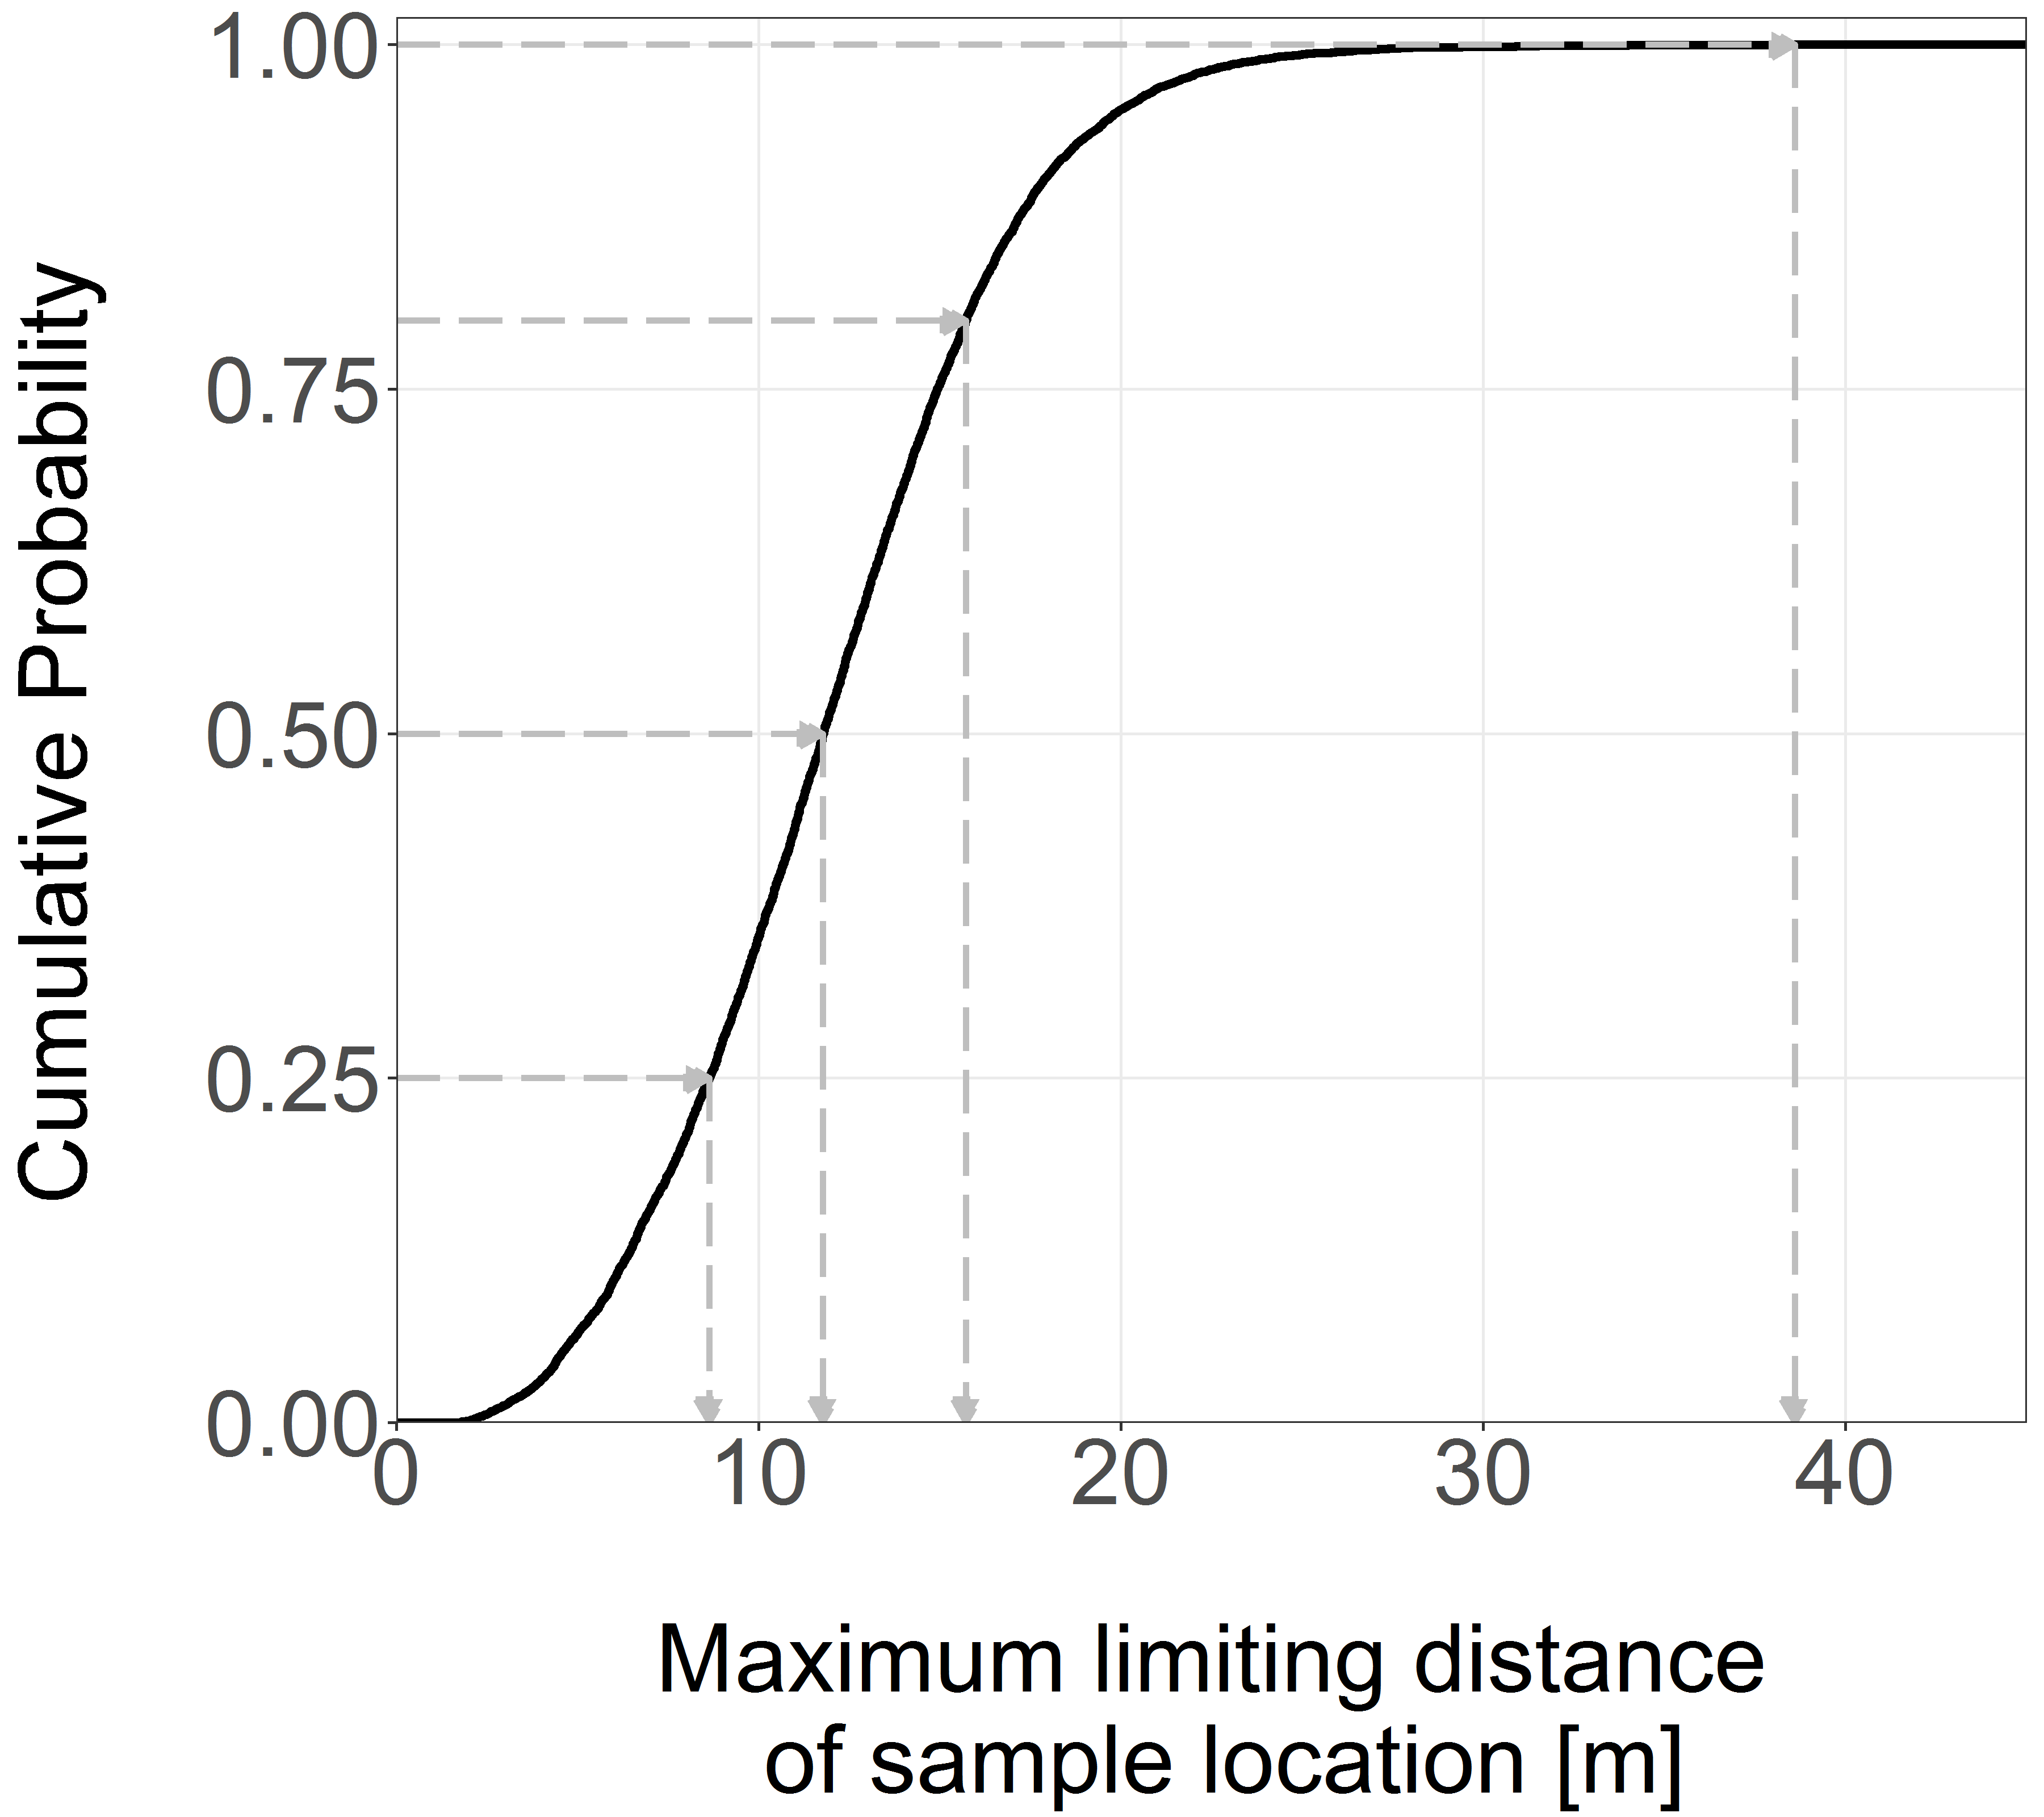
\includegraphics[width=0.36\textwidth]{Grafiken/Regmod_article/cdf_maxri.png}%
%	}\par\medskip
%	\subcaptionbox{Circular supports used to extract explanatory variables around sample locations. \textit{Dash dot dot line}: q100, \textit{dash dot line}: q80, \textit{dot dot line}: q50, \textit{dot line}: q25, \textit{solid line}: individual support, \textit{triangles}: sample trees \label{fig:sf2}}{
%		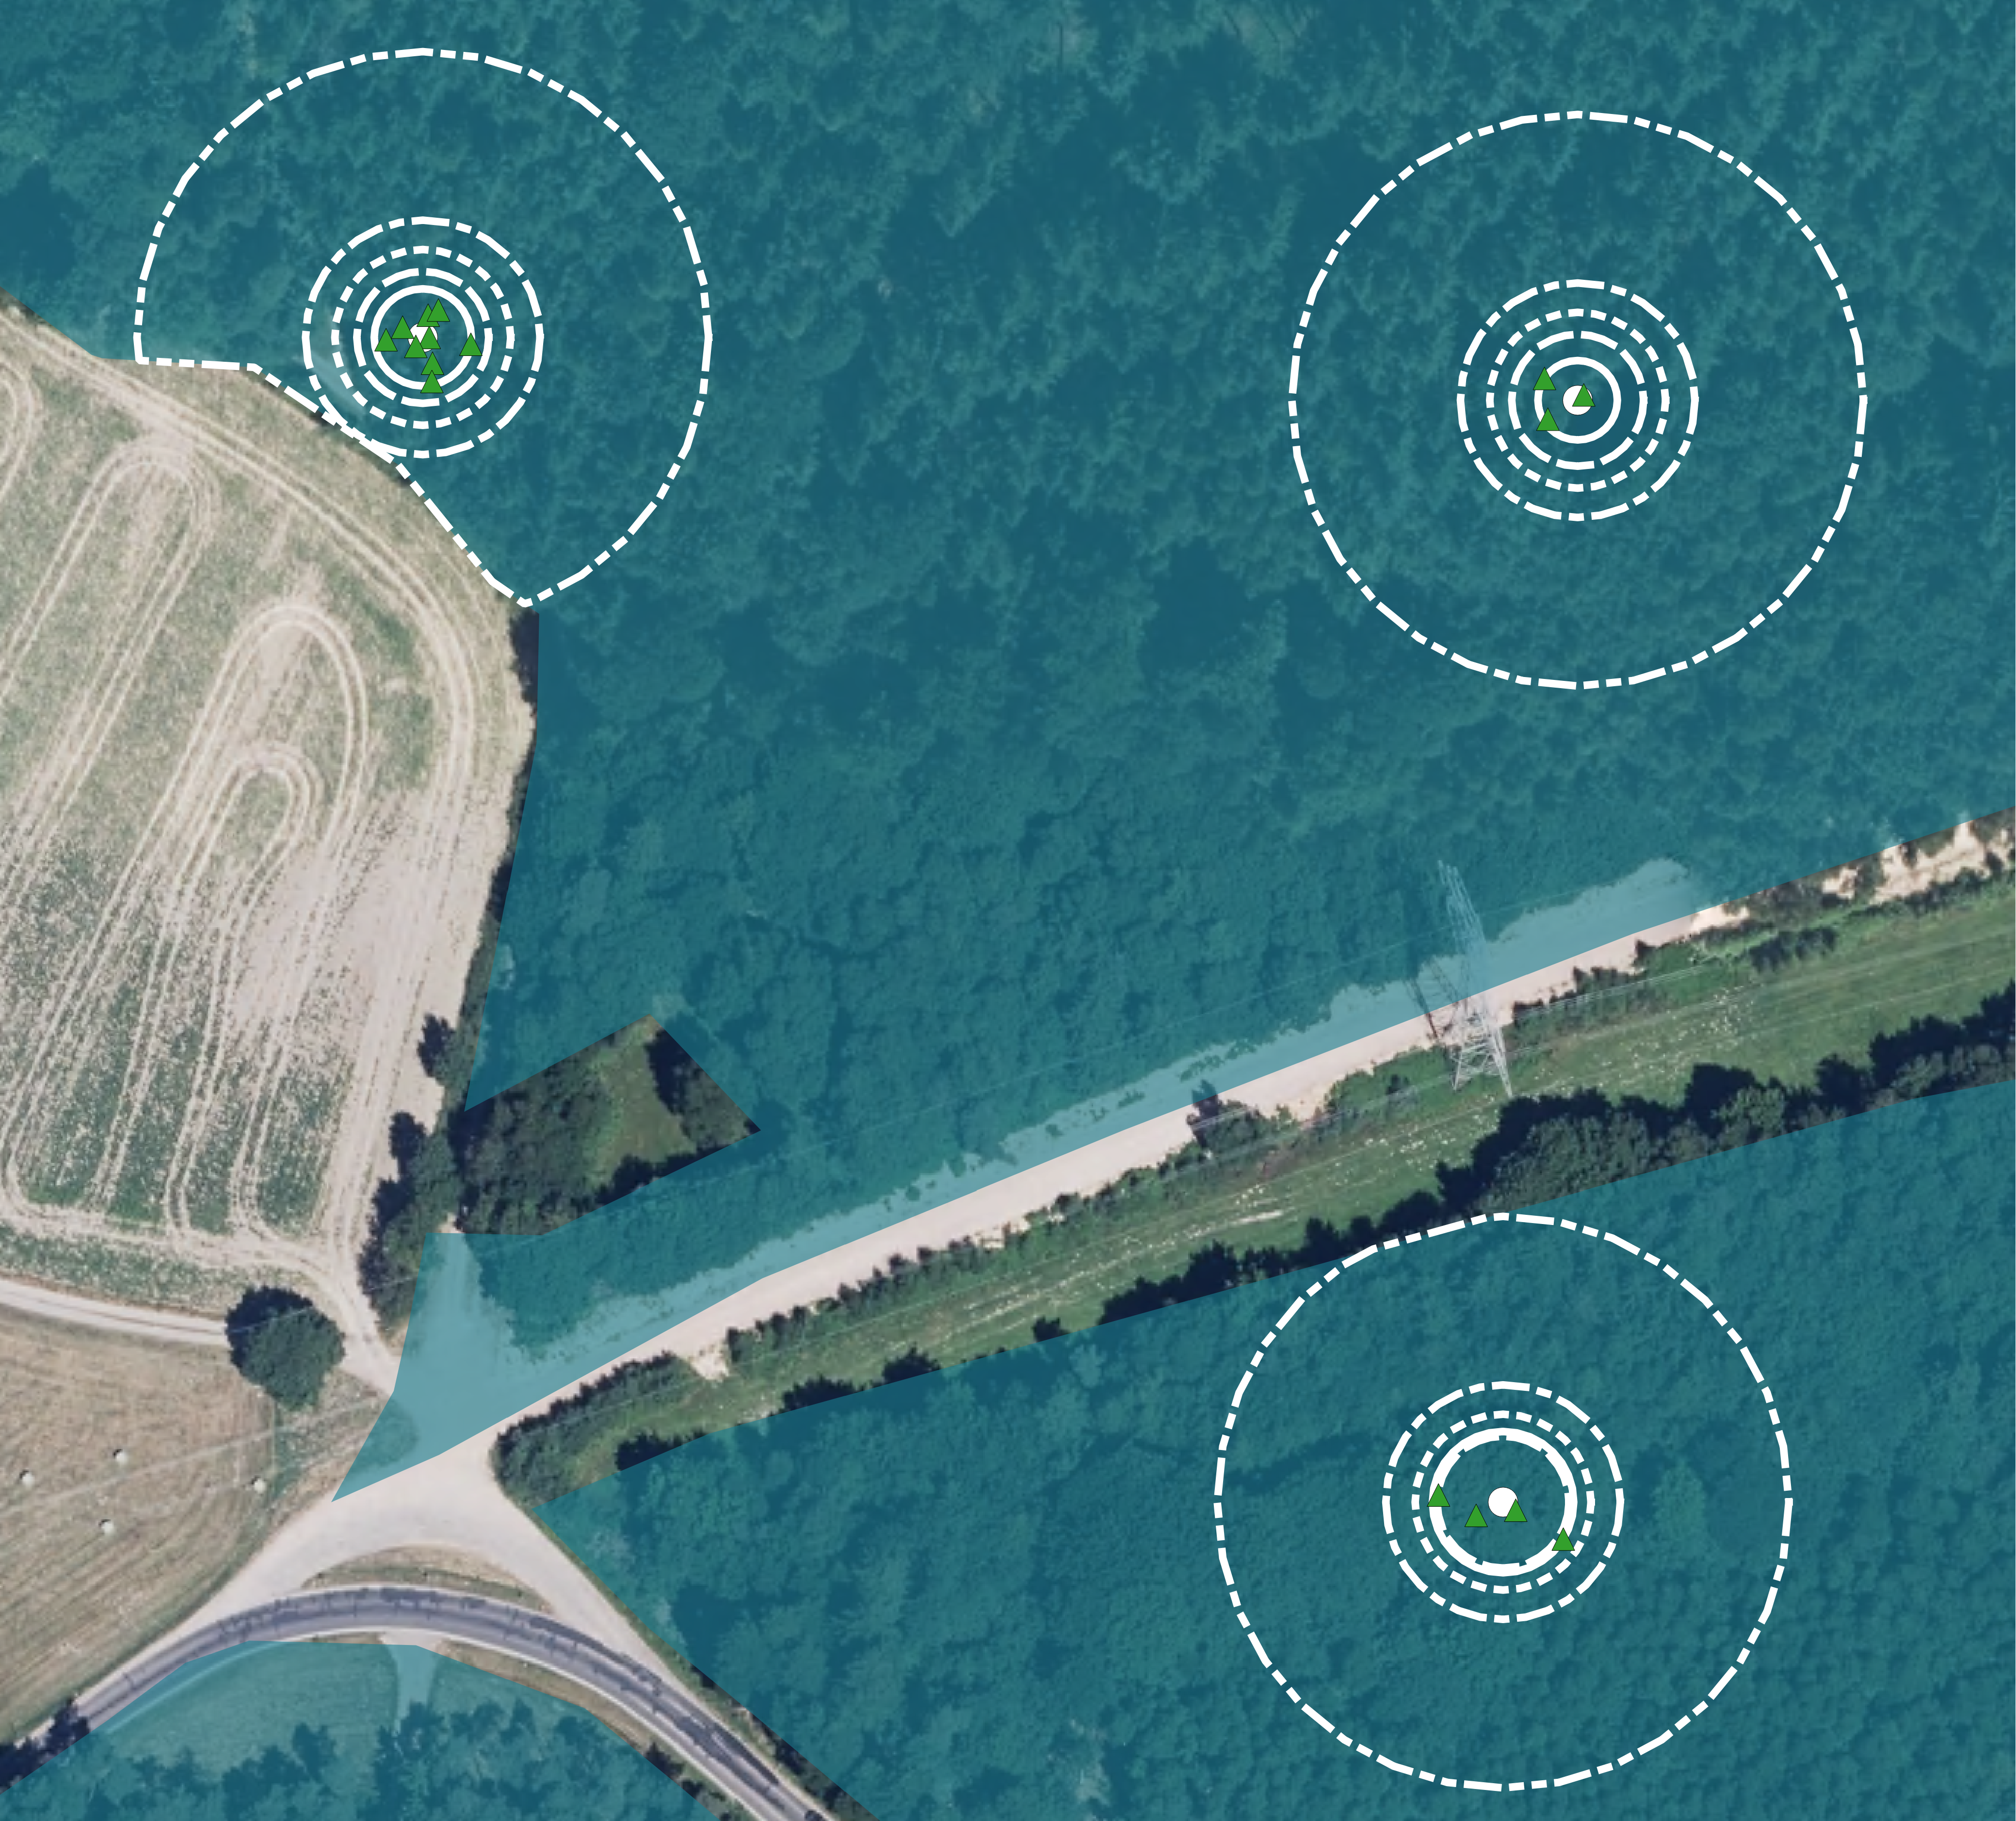
\includegraphics[width=0.36\textwidth]{Grafiken/Regmod_article/choice_of_support.png}
%	}\par\medskip
%	\caption{Identification (\textit{a}) and visualization (\textit{b}) of potential supports used for calculating the predictor variables on plot level}
%	\label{fig:tspec_supps}
%\end{figure}


\begin{figure}[h]
	\begin{subfigure}[t]{0.5\textwidth}
		\centering
		\resizebox{0.85\hsize}{!}{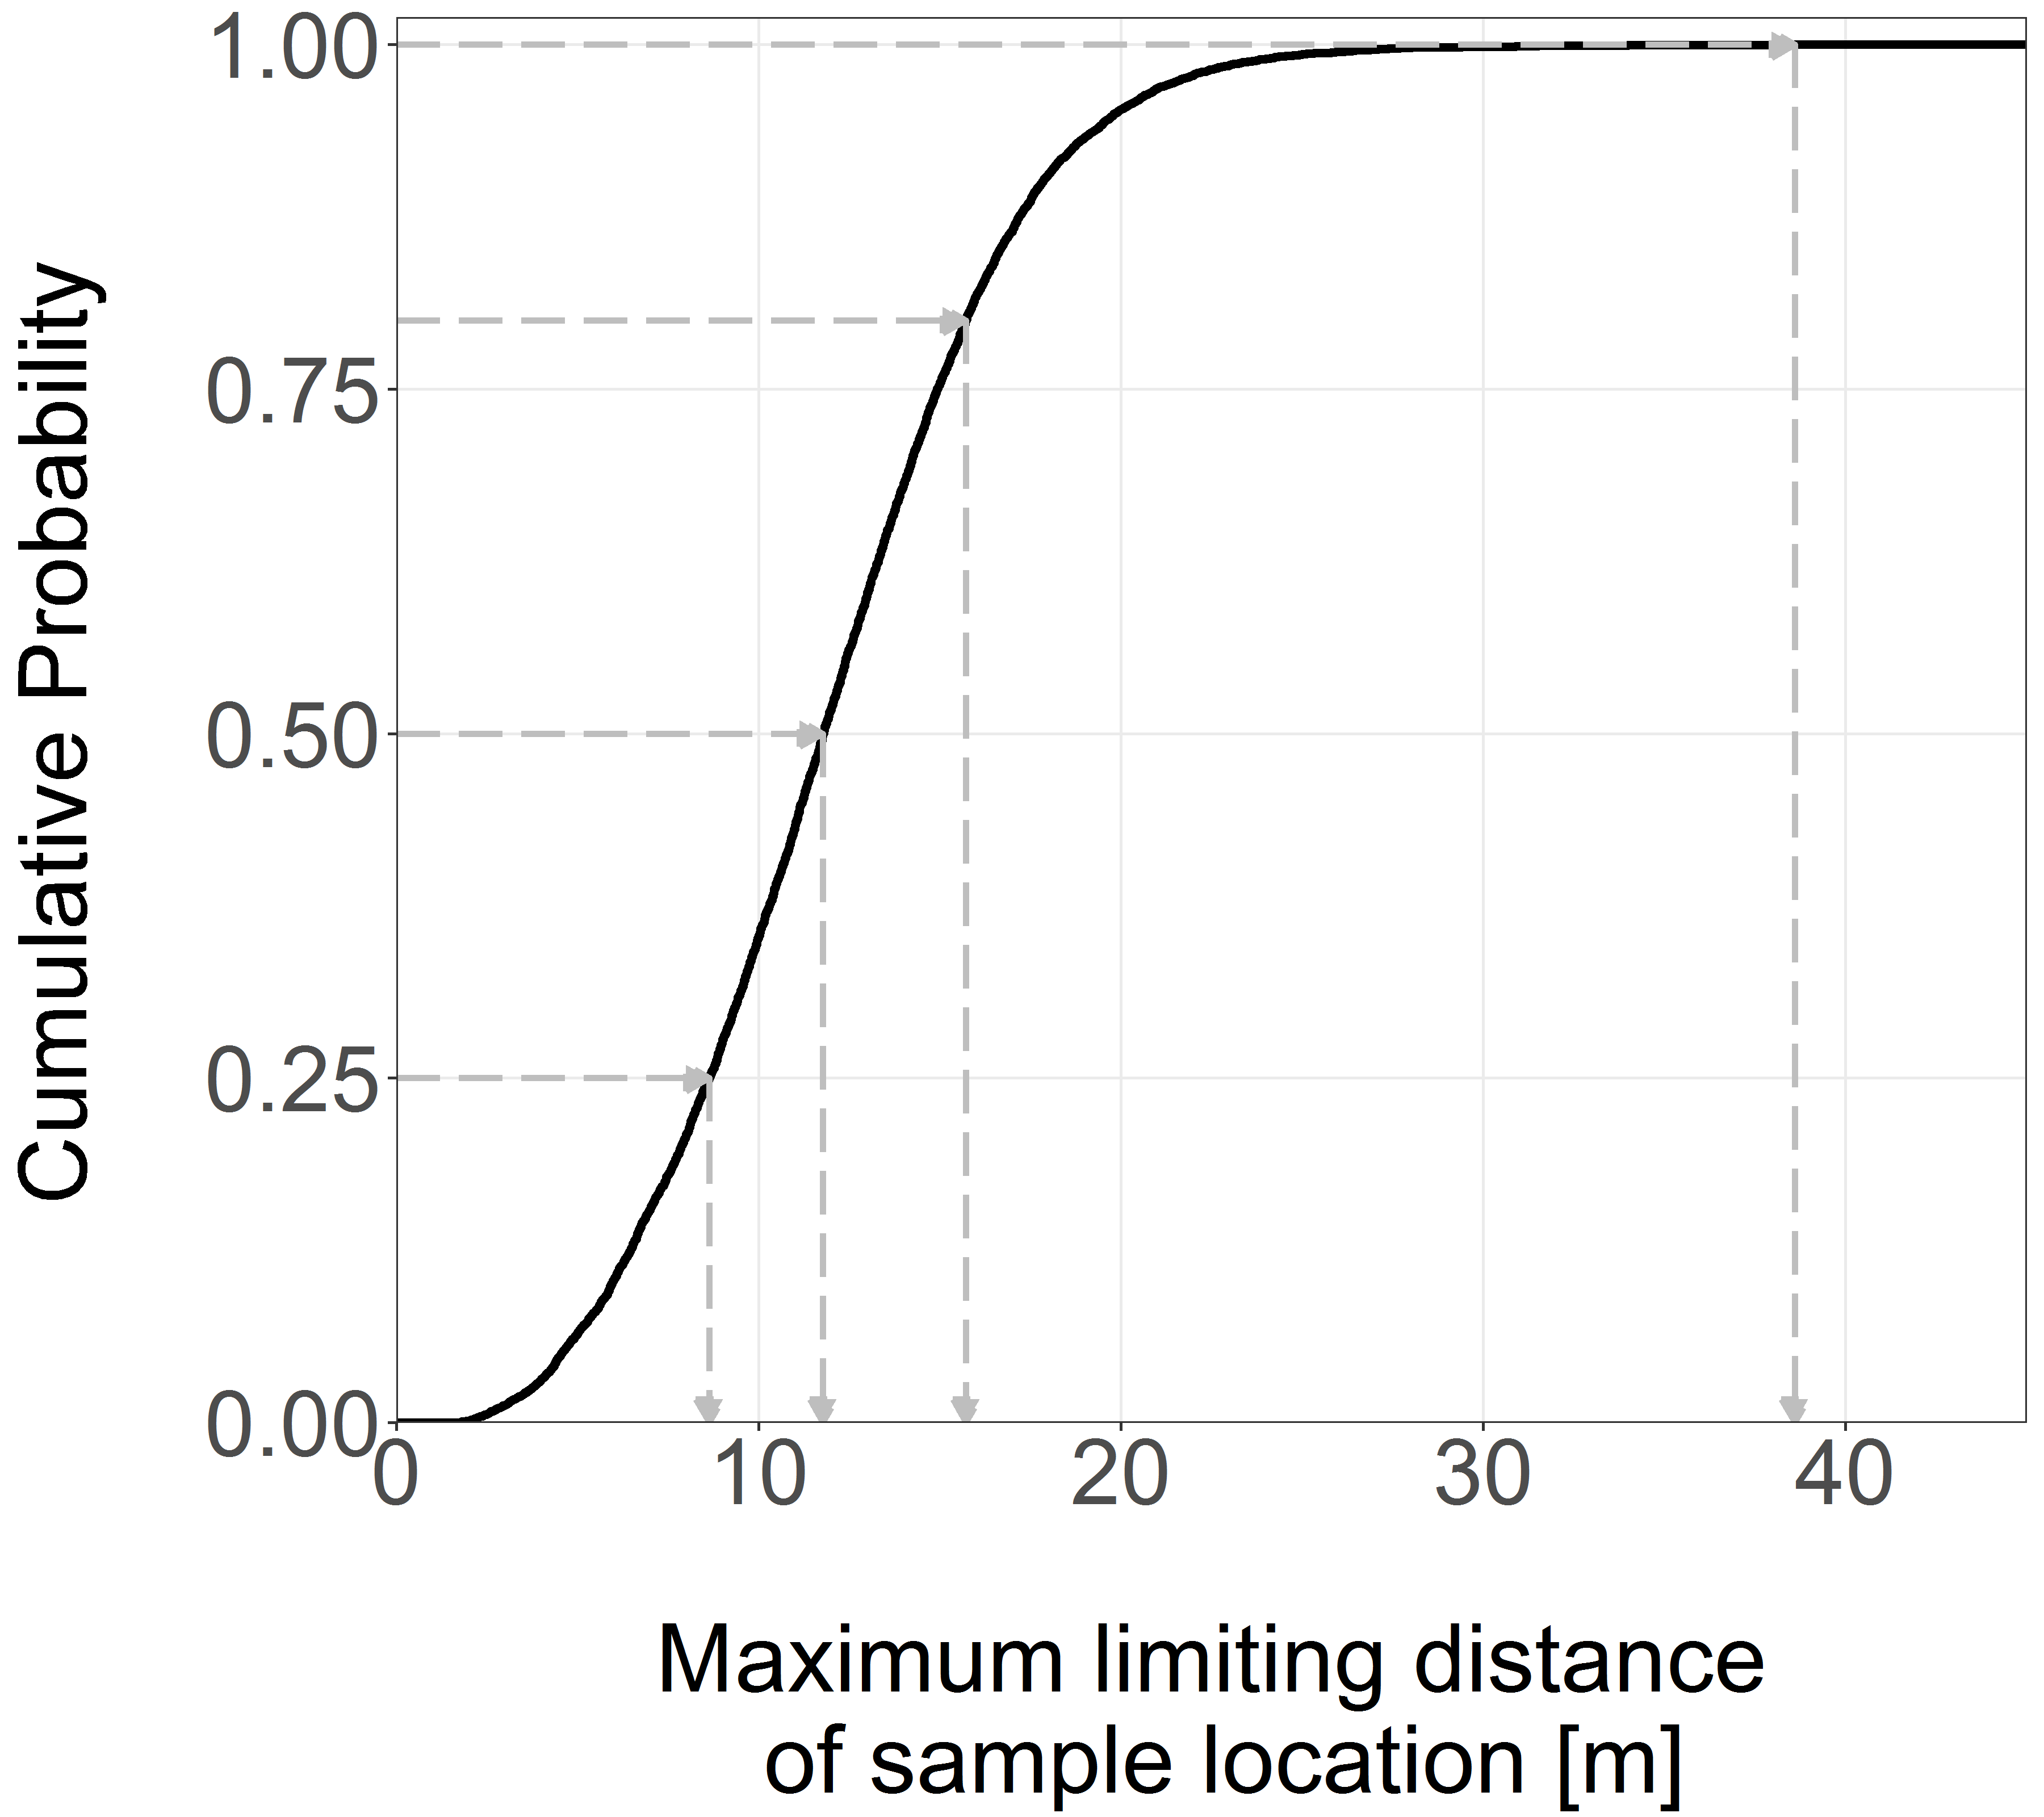
\includegraphics{Grafiken/Regmod_article/cdf_maxri.png}}%
		\caption{} \label{fig:sf1}
	\end{subfigure}
	\begin{subfigure}[t]{0.5\textwidth}
		\centering
		\resizebox{0.85\hsize}{!}{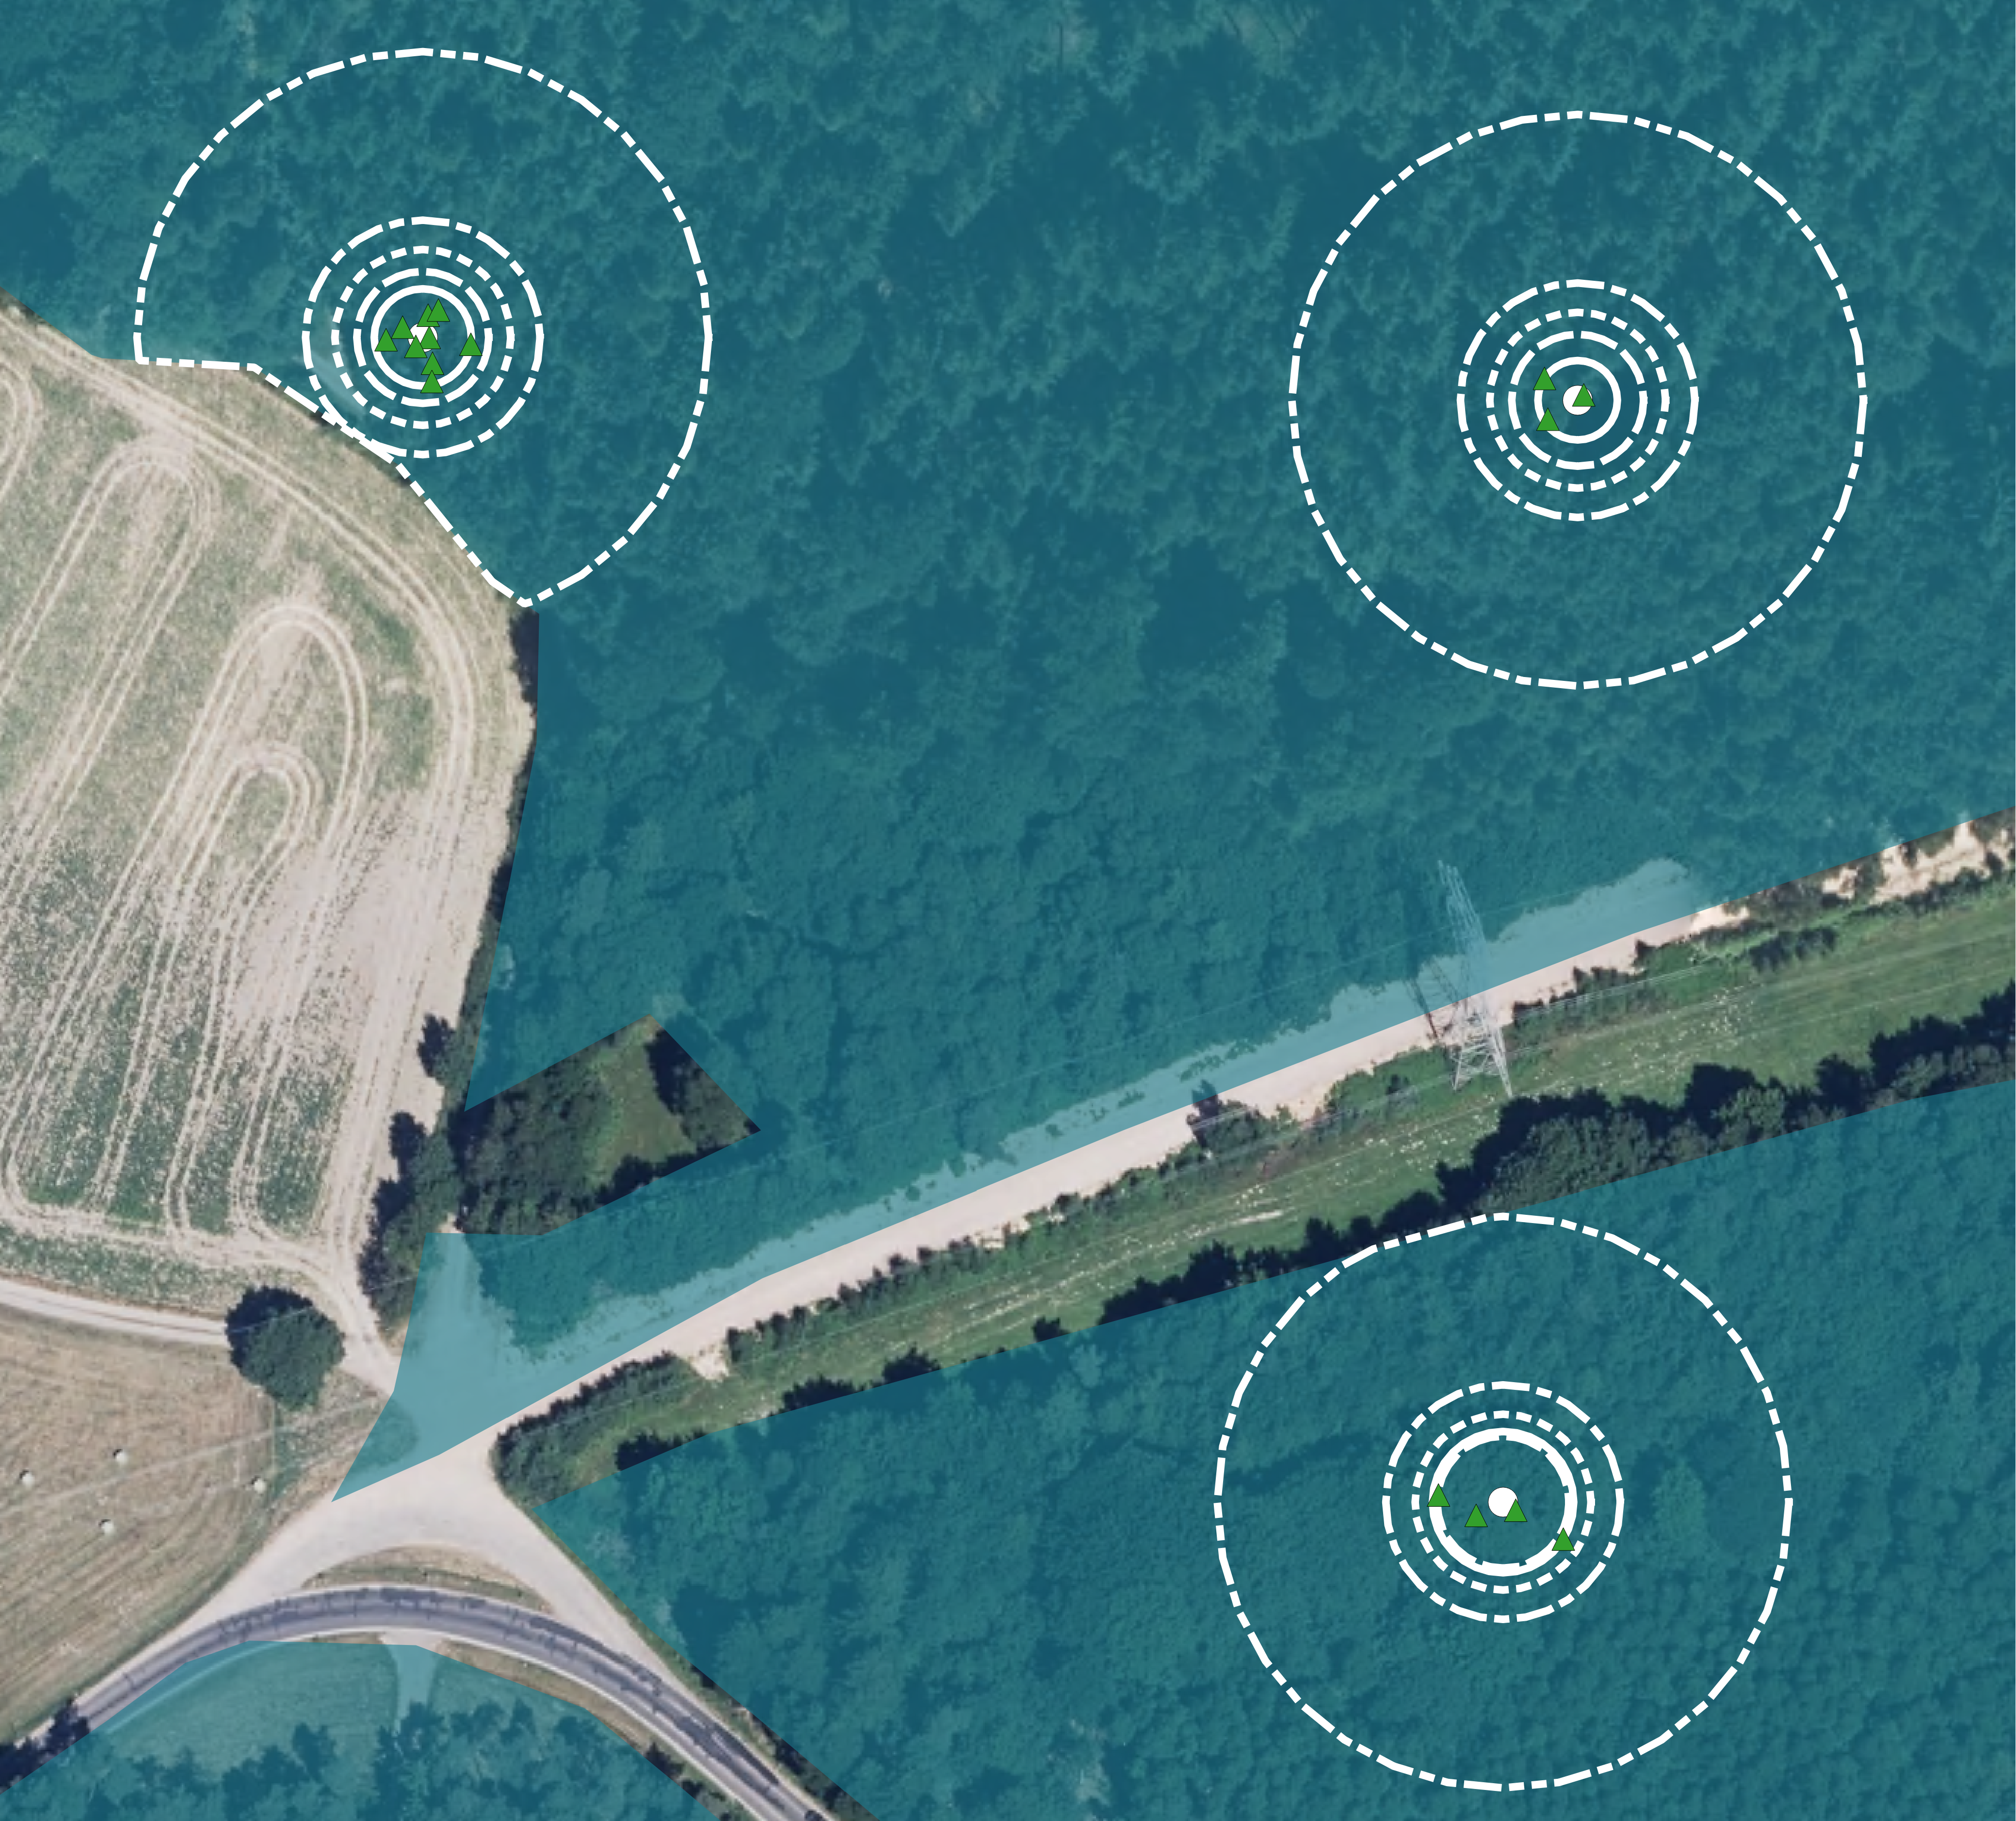
\includegraphics{Grafiken/Regmod_article/choice_of_support.png}}%
		\caption{} \label{fig:sf2}
	\end{subfigure}
     \caption{Identification (\textit{a}) and visualization (\textit{b}) of potential support radii used for calculating the predictor variables on plot level based on ECDF of maximum limiting distances of all \bwi{} sample locations in RLP.}
      \label{fig:tspec_supps}
\end{figure}

% ----------------------------------------------------------------------- %
% ----------------------------------------------------------------------- %
\subsection{\changed{Model Building and Evaluation}}
\label{sec:modval}

\changed{In order to judge the quality of the \textit{treespecies} variable, the user's accuracy for each classified species category and the overall accuracy of the classification scheme was calculated based on the confusion matrix \citep{congalton2008}. As reference data, we calculated the actual main plot tree species by applying the respective threshold to the sample trees of each sample plot.} The classification accuracy was evaluated for all support sizes for both the calibrated and the uncalibrated \textit{treespecies} variables. The measures of the regression model accuracy using both CHM- and $treespecies$ variables were defined as the 10-fold cross-validated root mean square error (\rmsecv{}, equation \ref{eq:RMSE}) and the adjusted coefficient of determination (\adjrsq{}) of the multiple linear regression model defined in equation \ref{eq:chmtspec_fullmod_term}. Additionally, we considered the interaction terms \textit{meanheight}:\textit{treespecies}, \textit{meanheight$^{2}$:treespecies}, \textit{meanheight}:\textit{ALSyear}, \textit{stddev}:\textit{ALSyear} and \textit{meanheight}:\textit{stddev} and performed a variable selection based on the Akaike Information Criterion (AIC) \citep{Akaike2011} in order to minimize the number of variables in the model. Due to a pronounced unbalanced design in the \textit{treespecies}-\textit{ALSyear} strata (Online Resource 2), no interaction between \textit{treespecies} and \textit{ALSyear} was possible. We evaluated the model for all support combinations, considering the use of individual support sizes for each auxiliary information, using both the calibrated and the uncalibrated \textit{treespecies} variable. The calibration model (Section \ref{sec:tspecclass}) for the \textit{treespecies} variable was recalculated for each respective support-threshold setting. 206 sample plots included no sample trees and the timber volume density $Y(x)$ was thus set to \textit{zero}. These \textit{zero-plots} were removed from the modeling dataset since they acted as leverage points in cases where the ALS height metrics were recorded long before the terrestrial survey. Together with the missing tree species information (Section \ref{sec:tspecclass}), the modeling dataset $s$ was limited to $n$=\changed{5171} observations.

\begin{subequations}\label{eq:RMSE}
	\begin{align}
	RMSE &= \sqrt{\frac{\sum_{x \in s}\big(\hat{Y}(x)-Y(x)\big)^2}{n}} \label{eq:RMSEa}\\
	RMSE\% &= \frac{RMSE}{\frac{1}{n}\sum_{x \in s}Y(x)}	\label{eq:RMSEb}
	\end{align}
\end{subequations}


\begin{equation} \label{eq:chmtspec_fullmod_term}
\begin{split}
Y(x) = &\beta_{0} + \beta_{1} \cdot meanheight + \beta_{2} \cdot meanheight^{2} + \\ 
&\beta_{3} \cdot stddev + \\
&\beta_{4} \cdot ALSyear_1 + ... + \beta_{12} \cdot ALSyear_9 + \\
&\beta_{13} \cdot treespecies_1 + ... + \beta_{18} \cdot treespecies_6 + \varepsilon(x)
\end{split}
\end{equation}



%-------------------------------------------------------------------------------------------%
% ---------------------------------- Results ---------------------------------------------- %

\section{Results}
\label{sec:Res}

% ----------------------------------------------------------------------- %
% ----------------------------------------------------------------------- %
\subsection{Classification Accuracies}
\label{sec:supp_tspec_res}

\subsubsection*{Effect of Support Size and Threshold}

Evaluating the uncalibrated tree species predictions revealed a dependency of the classification accuracies on both the applied threshold and the support size. Firstly, increasing the threshold led to a decrease in the user's accuracies for most of the tree species independent of the support choice (Fig. \ref{fig:cos_oaa_ua}). The reason for this is that raising the threshold to higher values leads to a higher probability for the reference class than for the predicted class to be assigned as class 'Mixed'. This is due to the distinct difference in the spatial resolution between the reference and prediction data: the rather coarse spatial resolution of the tree species raster map causes the predicted class to remain classified as one of the five tree species much longer than the reference data, which consist of individual sample trees of a sample location. This effect is amplified by high thresholds. The probability of the predicted class to also be classified as 'Mixed' can however be raised by increasing the number of raster cells to be evaluated. For this reason, the user's accuracies improve when using larger support sizes, and this effect is most pronounced under high thresholds. This scale-threshold dependency of the user's accuracy particularly affects tree species that most commonly occur in mixed forest stands in Rhineland-Palatinate, i.e. \textit{Scots pine}, $oak$ and $beech$. The user's accuracies for tree species that are mostly prominent in pure forest stands ($spruce$, \textit{Douglas fir}) logically turned out to be much more robust to changes in the thresholds and support sizes. Among the uncalibrated tree species predictions, $beech$ and $spruce$ produced the best predictions achieving UAs of up to 70\% and 80\%.  Although the predictions for \textit{Douglas fir} and \textit{Scots pine} generally performed less well than $beech$ and $spruce$, similar UAs can be produced by adjusting the threshold and support choices. UAs for $oak$ never performed better than 50\%.

\begin{figure}[H]
	\centering
	\resizebox{0.397\hsize}{!}{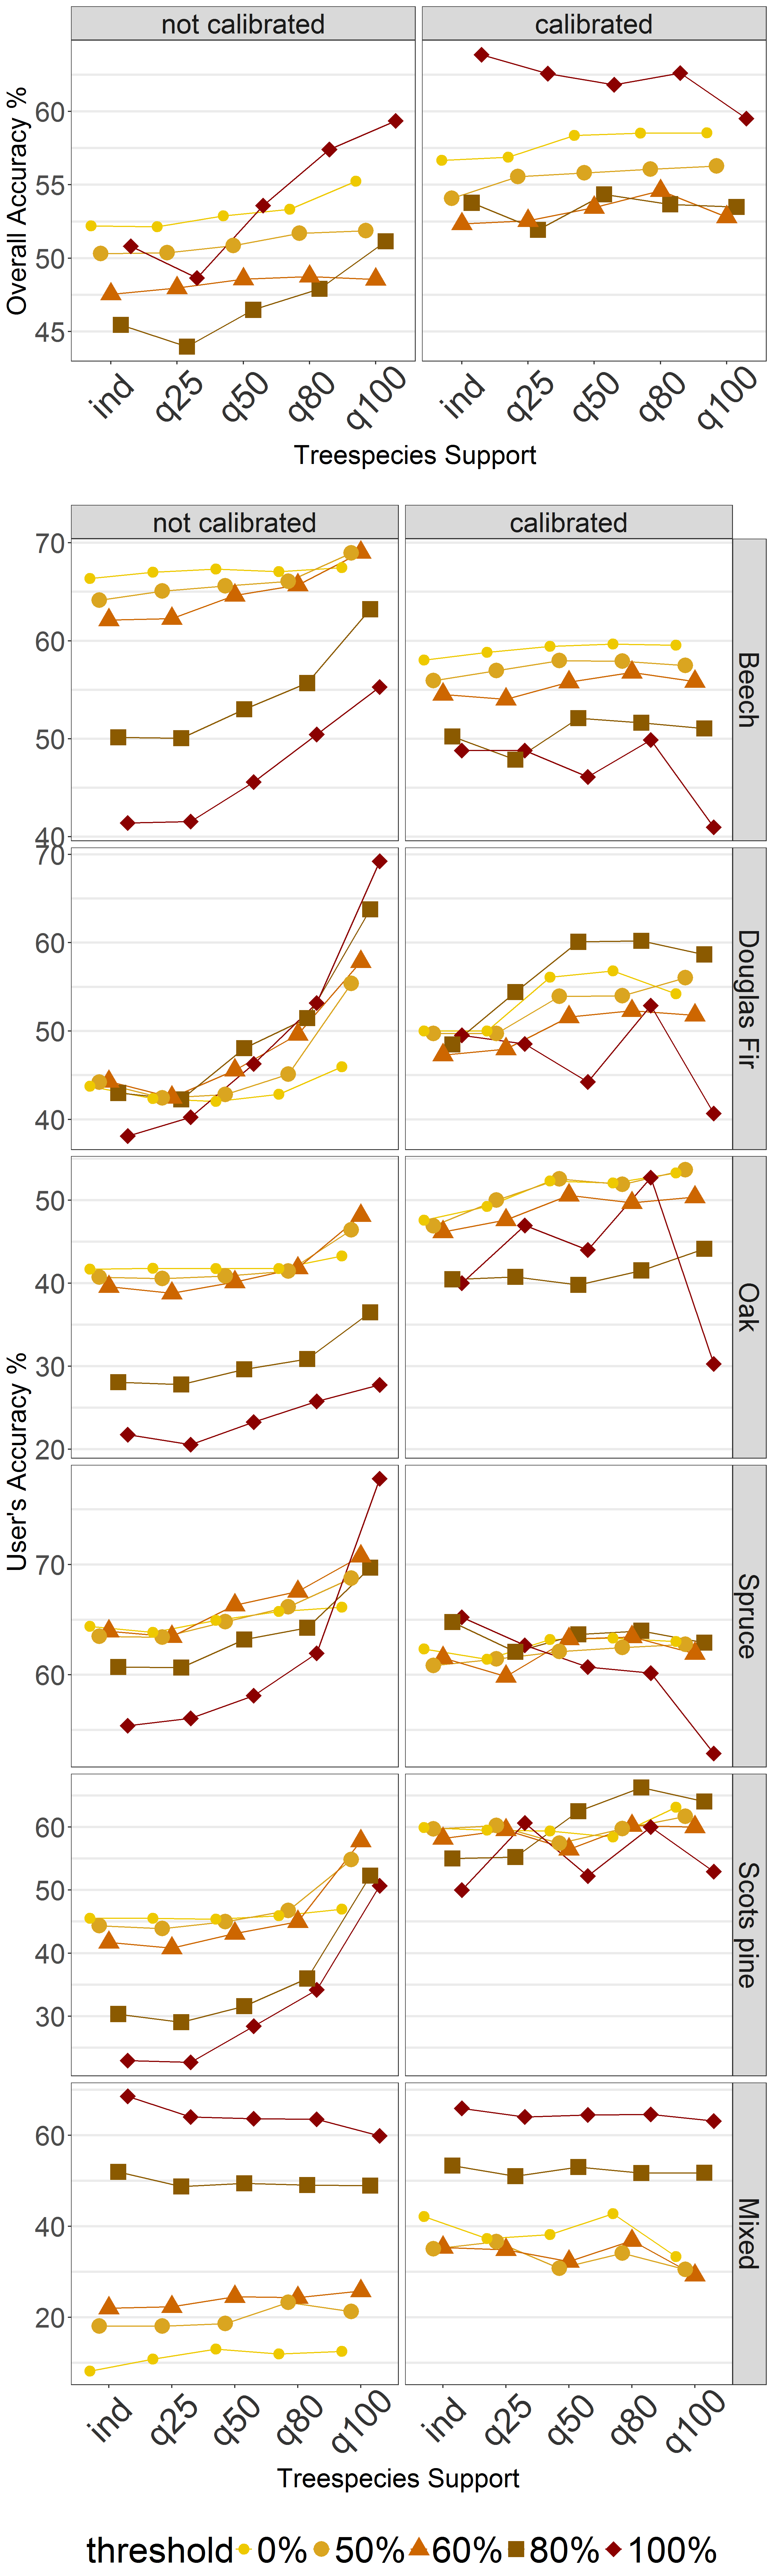
\includegraphics{Grafiken/Regmod_article/oaa_and_cos_tspec_mixed_cal_nocal.png}}
	\caption{Classification accuracy for the main tree species of a sample location \textit{before} and \textit{after} calibration: \textit{top)} overall accuracies. \textit{bottom)} user's accuracies. \textit{ind}: plot individual support sizes.}
	\label{fig:cos_oaa_ua}
\end{figure}


\subsubsection*{\changed{Calibration}}
Calibration substantially diminished the effect of the scale-threshold dependency for the five tree species and also increased the UAs for \textit{Scots pine} and $oak$. \changed{Whereas the UAs for $beech$ and $spruce$ were found to be slightly lower after calibration,} the overall accuracy under each support choice was always considerably increased by calibrating the tree species prediction (Fig. \ref{fig:cos_oaa_ua}). With respect to the calculated random forest models, the initial tree species prediction ($treespecies$) and the information about the growing region ($wgb$) turned out to be the most valuable information, followed by the estimated proportion of coniferous trees ($prop.conif$) and the mean canopy height ($meanheight$).


% ----------------------------------------------------------------------- %
% ----------------------------------------------------------------------- %
\subsection{Regression Model Accuracies}
\label{sec:supp_chm_tspec_res}


\subsubsection*{Effect of Support Size and Threshold}

Figure \ref{fig:supp_perf_res} shows the accuracies of the regression model (equation \ref{eq:chmtspec_fullmod_term}) achieved under all possible combinations of support sizes for the auxiliary data. The stepwise selection procedure always included all considered single and interaction terms. In terms of \adjrsq{} and \rmsecv{}, the analysis revealed that the choice of the CHM support size controls the overall level of the model's accuracy. The information about the main plot tree species can then be used to further improve the model fit under suitable $treespecies$ support and threshold settings. When using the uncalibrated $treespecies$ variable, an increase of the $treespecies$ support size causes an increase in the model performance if low thresholds are used, whereas high thresholds (80\%, 100\%) cause a decrease in the model performance. This threshold-dependency could be removed by calibrating the $treespecies$ variable. \changed{The highest \adjrsq{} and the lowest \rmsecv{} were realized using the $q50$ support for both the CHM and calibrated $treespecies$ variables in combination with a $treespecies$ threshold of 100\%, resulting in (\adjrsq{} of 0.48 and \rmsecv{} of 136.62 m$^2$/ha (43.8\%).} However, various support and threshold combinations for the CHM and $treespecies$ variables can be used to yield almost identical \rmsecv{} and \adjrsq{} values. A detailed table of the model accuracies is given in Online Resource 4.

\subsubsection*{Effect of Misclassifications}

\changed{We accessed the magnitude of the misclassification effect for all models that were analysed in Section \ref{sec:supp_chm_tspec_res}, i.e. for all possible support and threshold combinations for the CHM and $treespecies$ predictor variables. We first compared the \adjrsq{} of each model when using the uncalibrated $treespecies$ variable against the \adjrsq{} using the actual, i.e. error-free variable. We then did the same comparison for the model using the calibrated treespecies predictor variable. Figure \ref{fig:supp_r2_calnocal} provides a visualization of this comparison. Note that only the model with the predicted tree species variables can be applied to additional sample locations where no terrestrial survey has been carried out.} As expected, the highest \adjrsq{} for every evaluated model was always achieved using the error-free tree species variable, whereas the missclassifications in the tree species variable led to a systematic decrease of the model accuracy. The calibration of the initially predicted main plot tree species using the random forest classification algorithm (Section \ref{sec:tspecclass}) turned out to not only improve the classification accuracies (Section \ref{sec:supp_tspec_res}), but also to considerably decrease the effect of the missclassifications on the regression model predictions and accuracy. Figure \ref{fig:supp_r2_calnocal} ($right$) shows that the \adjrsq{} under the actual and the calibrated predicted tree species variable are in general much closer to, and in many cases even on the identity line. \added{The differentiation into two distinct point clouds results from the poor model performance under support size $q100$ for the CHM variables (i.e. the lower point cloud).} Whereas the misclassifications in the uncalibrated $treespecies$ variable led to a residual inflation of \changed{0.01 - 0.05} in \adjrsq{}, it was only between \changed{0 and 0.01} after calibration. Further analysis revealed that when using the calibrated $treespecies$ variable, the regression coefficients were almost identical to the ones received using the actual main plot tree species.

\begin{figure}[h]
	\centering
	\resizebox{1\hsize}{!}{\includegraphics*{Grafiken/Regmod_article/cos_cal_nocal_bw.png}}
	\caption{10-fold \rmsecv{}[\%] and \adjrsq{} realized under various support choices for the CHM and $tree species$ explanatory variables}
	\label{fig:supp_perf_res}
\end{figure}


\begin{figure}[h]
	\centering
	\resizebox{0.75\hsize}{!}{\includegraphics*{Grafiken/Regmod_article/cos_r2_cal_vs_nocal.png}}
	\caption{Effect on the \adjrsq{} when substituting the actual main tree species with the predicted  main tree species of a sample plot. Each point in the graph represents the timber volume regression model under different supports and threshold settings. The \textit{dotted} line tracks the the model with the highest \adjrsq{} under the use of the error-free \textit{treespecies} variable. Semitransparent colours for the data points are used to visualize overlap.}
	\label{fig:supp_r2_calnocal}
\end{figure}


% ----------------------------------------------------------------------- %
% ----------------------------------------------------------------------- %
\subsection{Final Regression Model}
\label{sec:regmod_final}

In order to address research questions 1 and 2 (i.e. the gain in model accuracy by tree species information and effect of heterogeneity in the ALS data), we investigated the model properties in more detail. For this purpose, we decided to use the best found model that was achieved under the support settings of $q50$ for both auxiliary data with a threshold of 100\% for the tree species variable as the regression model of choice. The reason for inspecting this model was that \textit{a)} the model provided the highest \adjrsq{} among all validated models while reducing the data handling complexity for upcoming applications (i.e. identical support sizes for all remote sensing data) and \textit{b)} the calibration neutralized the effects of misclassifications on the model predictions. The interaction term between $meanheight^2$ and $treespecies$ (i.e. considering separate curvatures for each tree species) turned out not to have a significant influence on the model accuracy and was dropped, resulting in an \adjrsq{} of 0.48 and a slightly increased \rmsecv{} of 140.62 m$^2$/ha (46.7\%). \added{The final model thus comprised 39 parameters (regression coefficients), i.e. the intercept, 3 main effects for continuous variables, 13 main effects for categorical variables and 22 interaction parameters (Table \ref{tab:modacc_modterms}).\par
	We also conducted an analysis for detecting influential data points or outliers for the final regression model. We here considered the commonly applied criteria of leverages and Cook's Distance as amongst others described in \citet[p. 160-167]{fahrmeir2013}. The critical threshold of $2p/n$ (i.e. twice the average of the hat matrix' diagonal entries) was exceeded by 10\% of the observations. However, only 3\% of these leverage points were assigned to studentized residuals with values $>$ 1 or $<$ -1. Removing these observations from the dataset and refitting the model led to an \adjrsq{} of 0.49 compared to 0.48 when including them. Additionally, Cook's Distance values $D_i$ did not exceed a value of 0.019, and were thus far apart from the commonly used critical threshold of $D_i >$ 0.5 that indicate a considerably change of the regression model results when omitting them. We thus decided not to remove any observations from the modelling dataset. We thus decided not to remove any observations from the modelling dataset.}

\begin{figure}[h]
	\centering
	\resizebox{0.91\hsize}{!}{\includegraphics*{Grafiken/Regmod_article/predlines_tspecaux_cal.png}}
	\caption{Visualization of the timber volume prediction function (\textit{final regression model}) on sample plot level for each main plot tree species and ALS acquisition year. For visualization purposes, the predictor variable $stddev$ was set to its average value within the respective \textit{treespecies} and \textit{ALSyear} categories. The terrestrially observed timber volume values are plotted in the background.}
	\label{fig:predlines_tspec}
\end{figure}

% latex table generated in R 3.4.2 by xtable 1.8-2 package
% Sun Jan 07 17:11:26 2018
\begin{table*}[!htbp]
	\centering
	\caption{Accuracy specifications for submodels of final OLS regression model. $p$ gives the number of parameters for each model. Interaction terms are indicated by ':'.} 
	\label{tab:regmod:mt}
	\begin{tabular}{llrrrr}
  \hline
model terms & model & $p$ & $R^2_{adj}$ & $RMSE_{cv}$ & $RMSE_{cv}\%$ \\ 
  \hline
  meanheight + stddev + meanheight$^2$ + \\ treespecies + ALSyear + \\ meanheight:treespecies + \\ meanheight:ALSyear + meanheight:stddev \\ + stddev:ALSyear & Final model &  39 & 0.48 & 140.62 & 46.69 \\ \\
  meanheight + stddev + meanheight$^2$ + \\ meanheight:stddev & Submodel 1 &   5 & 0.36 & 155.54 & 51.65 \\ \\
  meanheight + stddev + meanheight$^2$ + \\ ALSyear + meanheight:ALSyear + \\ meanheight:stddev + stddev:ALSyear & Submodel 2 &  29 & 0.45 & 145.62 & 48.35 \\ \\
  meanheight + stddev + meanheight$^2$ + \\ treespecies + meanheight:treespecies + \\ meanheight:stddev & Submodel 3 &  15 & 0.40 & 150.32 & 49.92 \\ 
   \hline
\hline
\end{tabular}
\end{table*}
%\endgroup


%% old version
%\begin{table*}
%	\centering
%	\caption{Accuracy metrics for submodels of final OLS regression model} 
%	\label{tab:modacc_modterms}
%	\begin{tabular}{llrrr}
%		\hline
%		model terms & model & parameters & $R^2_{adj}$ & \rmsecv{} \\ 
%		\hline
%		meanheight + stddev + meanheight$^2$ + \\ treespecies + lidaryear + meanheight:treespecies + \\ meanheight:lidaryear + meanheight:stddev + \\ stddev:lidaryear & final model &  39 & 0.49 & 132.12 \\ \\
%		meanheight + stddev + meanheight$^2$ + \\ meanheight:stddev & submodel 1 &   5 & 0.35 & 148.03 \\ \\
%		meanheight + stddev + meanheight$^2$ + \\ lidaryear + meanheight:lidaryear + \\ meanheight:stddev + stddev:lidaryear & submodel 2 &  29 & 0.44 & 137.52 \\ \\
%		meanheight + stddev + meanheight$^2$ + \\ treespecies + meanheight:treespecies + \\ meanheight:stddev & submodel 3 &  15 & 0.41 & 137.52 \\ 
%		\hline
%		\hline
%	\end{tabular}
%\end{table*}
%%\endgroup

\subsubsection*{Interpretation of Final Regression Model}
\label{sec:prop_regmod_final}
Figure \ref{fig:predlines_tspec} provides a visualisation of the timber volume predictions separated by the calibrated tree species and the ALS acquisition years. Sample plots classified as $oak$ and \textit{Scots pine} revealed to have an almost identical relationship (nearly identical slopes) for the mean canopy height - timber volume relationship. They only differ by a marginally higher intercept for \textit{Scots pine} plots, meaning that given the same mean canopy height a sample plot dominated by \textit{Scots pine} yields a marginally higher timber volume on the plot level than a plot dominated by $oak$. $Beech$-dominated sample plots tend to achieve a higher timber volume than $oak$ and \textit{Scots pine} for canopy heights below 20 meters, but realize the lowest timber volumes for canopy heights above 20 metres. Sample plots dominated by any of the remaining coniferous tree species (\textit{Douglas fir}, $spruce$) revealed to have higher slopes than broadleaf classified plots. This indicates that given the same mean canopy height, sample plots dominated by \textit{Douglas fir} and $spruce$ yield higher timber volume values than broadleaf- or \textit{Scots pine} dominated sample plots, and this difference becomes more pronounced with increasing mean canopy heights. Within the group of coniferous-dominated sample plots, $spruce$ turned out to have the highest slope, thereby yielding the highest timber volume values for mean canopy heights above 15 meters. An undesired characteristic of the model is that the predicted timber volume can in some cases ($<$ 1\%) take negative values for low canopy heights (e.g. for $spruce$-dominated plots with \textit{meanheight} below 5 meters and $stddev$ of 4 meters). \changed{However, we chose not to use a log-transformation of the response variable. Doing so would have prevented the subsequent calculation of the g-weight variance of the design-based estimators \citep{mandallaz2013a, mandallaz2013b}, which is only possible for response variables on the original scale. The g-weight variance provides the benefit of a better variance estimate for internal models by considering the dependency of the regression coefficients on the realized sample. The rare occurrence of negative predictions were however not considered to have an influence on subsequent design-based estimates when averaging multiple predictions within given spatial domains.}


\subsubsection*{Effect of Time-Lags and Heterogeneity in ALS Data}

Incorporating the ALS acquisition year as a categorical variable ($ALSyear$) in the regression model substantially accounted for the variability in the data introduced by \textit{a)} the time-lags between ALS acquisition and terrestrial survey, and \textit{b)} variation in ALS data quality which are due to sensor- and post processing techniques (Table \ref{tab:modacc_modterms}). \changed{Whereas the \adjrsq{} for the regression model without considering the ALS acquisition year as additional predictor variable (\textit{submodel 1}) was 0.36, it could already been increased to 0.40 by including the tree species variable (\textit{submodel 2}). A further stratification by the ALS acquisition year increased the \adjrsq{} of \textit{submodel 1} from 0.36 to 0.45, and the \adjrsq{} of \textit{submodel 3} from 0.40 to 0.48.}\par

We further analysed the model residuals within each ALS acquisition year (within-group variation) for the final model and nested submodels. It turned out that the $R^2$ values vary distinctly between the ALS acquisition year strata (Table \ref{tab:adj_r2_within}). More precisely, the within-group $R^2$ can be higher and lower than the overall $R^2$ of the respective model. Figure \ref{fig:r2adj_in_lyears} shows that a stratification according to the ALS acquisition years (submodel 2) can already increase the $R^2$ in most acquisition year strata, compared to the basic model using only the ALS height metrics as predictor variables (submodel 1). In the ALS acquisition year stratum 2007, the increase in $R^2$ even reached 0.08.

% latex table generated in R 3.4.2 by xtable 1.8-2 package
% Sun Jan 07 17:26:28 2018
\begin{table}[ht]
	\centering
	\caption{$R^2$, RMSE and RMSE\% of final regression model within ALS acquisition year strata (\textit{ALSyear}). $Area_{ALSyear}$: Area covered by ALS acquisition given in km$^2$. \textit{n}: number of validation data.}
	\label{tab:regmod:adj_r2_within}
	\begin{tabular}{lllrrr}
		\hline
		\textit{ALSyear} & $Area_{ALSyear}$ & $R^2$ & RMSE & RMSE\% & n \\ 
		\hline
 2012 & 2807   & 0.61 & 135.84 & 44.87 & 408 \\ 
 2011 & 4361  & 0.57 & 146.21 & 48.29 & 883 \\ 
 2010 & 4182 & 0.51 & 120.90 & 39.93 & 1171 \\ 
 2009 & 2100 & 0.42 & 133.42 & 44.07 & 559 \\ 
 2008 & 2968 & 0.48 & 130.38 & 43.06 & 701 \\ 
 2008\_1 & 2116 & 0.33 & 175.43 & 57.94 & 394 \\ 
 2007 & 3498 & 0.46 & 136.47 & 45.08 & 418 \\ 
 2003 & 602 & 0.27 & 154.48 & 51.02 & 529 \\ 
 2002 & 775 & 0.44 & 141.55 & 46.75 & 314 \\ 
		\hline
\hline
\end{tabular}
\end{table}
%\end{longtable}
%\endgroup

%% old version
%\begin{table}[ht]
%	\centering
%	\caption{$R^2$, RMSE and Residual Square Sum (SSE) of final regression model within LiDAR acquisition year strata (\textit{lidaryear}). \textit{n}: number of validation data}
%	\label{tab:adj_r2_within}
%	\begin{tabular}{llrrr}
%		\hline
%		LiDAR acquisition year & $R^2$ & rmse & SSE & n \\ 
%		\hline
%		2012   & 0.55 & 139.54 & 7535278 & 387 \\ 
%		2011   & 0.55 & 145.21 & 17880553 & 848 \\ 
%		2010   & 0.48 & 122.16 & 16907662 & 1133 \\ 
%		2009   & 0.43 & 127.17 & 8652419 & 535 \\ 
%		2008\_1 & 0.34 & 170.49 & 11161424 & 384 \\ 
%		2008   & 0.50 & 124.39 & 10475374 & 677 \\ 
%		2007   & 0.49 & 129.72 & 6950192 & 413 \\ 
%		2003   & 0.32 & 146.37 & 11139814 & 520 \\ 
%		2002   & 0.43 & 139.79 & 6038601 & 309 \\ 
%		\hline
%		\hline
%	\end{tabular}
%\end{table}
%%\end{longtable}
%%\endgroup


\begin{figure}[H]
	\centering
	\resizebox{0.62\hsize}{!}{\includegraphics*{Grafiken/Regmod_article/r2adj_in_lyears.png}}
	\caption{$R^2$-values of the final regression model, submodel 1 and submodel 2 achieved $within$ the ALS acquisition year strata.}
	\label{fig:r2adj_in_lyears}
\end{figure}


\subsubsection*{Added Value of Tree Species Map Information}
\changed{Introducing the predicted main tree species of a sample plot as an additional categorical variable to submodel 2 yielded a further increase in the \adjrsq{} of 0.03 (Table \ref{tab:modacc_modterms}). However, the improvement was even more pronounced in ALS acquisition years close or identical to the year of the terrestrial inventory (Fig. \ref{fig:r2adj_in_lyears}). We observed an increase of 0.06 in $R^2$ for ALS acquisition year 2012, and of 0.07 for ALS acquisition year 2011.} The analysis illustrated once more that misclassifications in the tree species variable generally reduce model accuracy compared to using error-free tree species information. The residual inflations caused by the misclassifications in the uncalibrated $treespecies$ variable within the $ALSyear$ strata were up to 0.05 in R$^2$. However, the calibration was able to substantially decrease or even remove the effects of misclassifications on the model accuracy in all ALS acquisition year strata.


%----------------------------------------------------------------------------------------------%
% ---------------------------------- Discussion ---------------------------------------------- %

\section{Discussion}
\label{sec:Dis}

% ----------------------------------------------------------------------- %
% ----------------------------------------------------------------------- %
\subsection{Stratification according to ALS Acquisition Years and Tree Species}
\label{sec:strat_dis}

Incorporating the main tree species of a sample location in the timber volume regression model increased the model accuracy and revealed strong evidence for the existence of a tree species specific behavior concerning timber volume on the plot level. This result seems reasonable regarding the species specific taper functions on single-tree level applied in the \bwi{} \citep{kublin2003, kublin2013}. \added{These findings also agree with those of \citet{latifi2012} who found an almost identical improvement in RMSE of 2\% when stratifying to broadleaf and coniferous tree species. The overall RMSE of their model was however 10\% smaller than in our study. The overall RMSE of their model  was however 10\% smaller than in our study. This might be due to a more heterogeneous dataset of much smaller sample size in the cited study, but also because the temporal alignment between the auxiliary data acquisition and the terrestrial survey was much better than in our case. Additionally, the number of different tree species present in their dataset was lower than in our case and only comprised Scots pine, European beech and oak. The individual effects of spruce and Douglas fir indicated by our model also support the findings of \citet{breidenbach2008}, who found a higher percentage of coniferous trees in a sample plot to increase the timber volume predictions. This was not true for Scots pine and oak whose effects turned out to be very similar for our dataset. However, in our study the stratification according to the ALS acquisition years severely limited the flexibility of species-specific prediction functions and model interpretability.} In particular, using the ALS acquisition years as categorical variables led to highly unbalanced datasets when stratifying according to the main plot tree species. This prevented the use of further stratification variables such as bioclimatic growing regions due to confounding effects and consequent singularities in the design matrices. \added{Using the ALS acquisition years as categorical variables also implied an artificial increase in the number of parameters in the OLS regression model, which was however not regarded as critical with respect to overfitting issues due to the high amount of observations used for fitting the regression coefficients \citep[Ch. 15.1]{draper2014}.} A stratification to the ALS acquisition years however proved to be an effective means in accounting for the artificially introduced noise in the data caused by quality variations and the large time-lags between the remote sensing and terrestrial data. \added{It allowed for a model accuracy that was very close to those reported by \citet{maack2016} who conducted a very similar study in the German federal state of Baden-W\"urttemberg.} Model accuracies were also particularly higher in ALS acquisition year strata in which the data showed considerably less noise or were closer to the date of the terrestrial survey. \added{This effect was significantly reduced or even removed when merging several ALS acquisition year strata. Promising steps with respect to more up-to-date canopy height information have already been made, as the topographic survey institution of RLP is currently processing a canopy height model from aerial imagery acquisitions for 2011 and 2012 covering the entire federal state. These aerial photography acquisitions will in the future be conducted in a two-year period, allowing to derive up-to-date canopy height information in the framework of future forest inventories. For a smaller study area, \citet{kirchhoefer2017} have already demonstrated that similar model accuracies for German NFI data can be achieved using imagery-based canopy height models.}\par

Incorporating the calibrated tree species information further improved the model accuracy by \changed{0.03} in adjusted R$^2$. Compared to the simple model only containing ALS height metrics, including the ALS quality and calibrated tree species information increased the adjusted $R^2$ by \changed{0.12} in total. A differentiated evaluation of the final regression model revealed that the highest R$^2$-values were achieved within ALS acquisitions year strata close or identical with the year of the terrestrial survey, showing differences of up to \changed{0.3} between the R$^2$s. Also the gain in R$^2$ by including the tree species information was largest (i.e. \changed{0.07}) in combination with ALS information acquired in the year of the terrestrial inventory. These insights were particularly interesting with respect to the further use of the regression model for small area estimations. Small area estimators generally gain modeling strength by defining the prediction model $globally$ (i.e. using all data in the inventory area), and then applying the so-derived prediction model to a subset of observations located within the area of interest \citep{mandallaz2013a}. Consequently, the proposed stratification technique in the prediction model is expected to yield a gain in model accuracy and a reduction of the small area estimation errors if the small area domain mostly includes data from strata that have high within-strata model accuracies. \added{Findings of \citet{breidenbach2008} indicated that a further increase in model accuracies could possibly be achieved when incorporating these categorical variables as random rather than fixed-effects in linear mixed-effects models \citep{pinheirobates2000}. The reason we did not apply this family of models was that small area regression estimators subsequently applied in RLP \citep{mandallaz2013a, mandallaz2013b} require the internal models to be fitted by OLS technique.}\par


% ----------------------------------------------------------------------- %
% ----------------------------------------------------------------------- %
\subsection{Calibration of Tree Species Map Information}
\label{sec:calib_dis}
The accuracy assessment of the initially derived main plot species from the classification map revealed the presence of misclassifications that led to a decrease in model accuracy. \added{This is in agreement with the potential effects of erroneous explanatory variables discussed in \citet{carroll2006} and \citet{gustafson2003}, i.e. an increase of variability (noise) in the data that can increase the amount of unexplainable variance and thereby reduce the model accuracy.} One reason for the misclassifications were that the classification algorithm of \citet{stoffels2015} was exclusively trained in pure stands with the objective to predict the \textit{dominant tree species} of a forest stand. Thus, our requirements on the classification map differed considerably from the ones imposed by \citet{stoffels2015} and have to be considered as far more difficult to meet. Firstly, the reference data used in the accuracy assessment also included understory trees that were recorded in the \bwi{} sample. Secondly, determining an exact spatial validation unit for a sample location (support) is not possible due to the properties of angle count sampling (Section \ref{sec:supp}). Thirdly, distinct discrepancies in the spatial scale between the reference data and the classification map severely hamper exact predictions of the main plot tree species especially in mixed forest stands. The latter issue caused a pronounced dependency of the user's accuracy on the support and threshold choice, particularly for tree species that most commonly occur in mixed forest structures, i.e. \textit{Scots pine} (91\%), $oak$ (90\%) and $beech$ (85\%) \citep{bwi3}. With respect to this set-up, the application of our calibration method proved to be of high value. It led to an increase in the classification accuracies, particularly for those tree species that performed worse in the uncalibrated setup, and thereby successfully minimized and even removed the deleterious effect of misclassifications on model accuracy and regression coefficients. Whereas the extensive analysis in our study deepened the understanding of the afore mentioned scale-effects, an alternative method for future applications could be to use map-derived percentages of each tree species as predictor variables in the random forest algorithm in order to directly predict the terrestrially observed main plot tree species.


% ----------------------------------------------------------------------- %
% ----------------------------------------------------------------------- %
\subsection{Choice of Support under Angle Count Sampling}
\label{sec:supp_choice_dis}

\changed{The validation of different support sizes underlined that the support choice can impact the accuracy of a prediction model, and thus confirmed the findings of \citet{deo2016}. In the present study, differences in the model accuracies however turned out to be small for most support choices. An exception was the choice of the $q100$ support for the CHM derived variables (38 meter radius), where the model accuracy was considerably worse than under the optimal settings. Contrary to our hypothesis, the use of plot-individual supports did not yield the best prediction performance overall. \citet{kirchhoefer2017} recently came to the same result when they transferred the angle-count sampling technique to a pixel-wise selection method of the auxiliary data that resembles the sample tree selection even more precisely. In their study, the application of fixed support sizes did also not perform worse than under variable supports. We consider two plausible reasons for the joint findings: first, the determination of an exact spatial extent that can be transferred to auxiliary data extraction remains technically infeasible under angle count sampling. Thus, angle count sampling does not seem to be adequate when linking inventory information with remote sensing data. Secondly, inaccuracies in the DGPS-measurements of the plot center locations as reported by \citet{lambrecht2017} may have an increased impact on the model accuracy the more exact the auxiliary data derivation spatially corresponds to those of the field survey. However, the extensive analysis carried out in our study also indicated that the optimal support size does not only depend on the spatial extent of the field plots, but also on the spatial resolution of the remote sensing data as well as the context in which the derived information is used in the prediction model. In the case of transforming the tree species information map into a suitable categorical predictor variable, the use of a large support size of 38 meter radius turned out to yield the best model accuracy. However, only few sample locations in the study area were actually characterized by limiting circles of that particular size. An analysis to find the best support settings therefore seems to be advisable prior to further applications of design-based or model-dependent inventory methods so as not to lose model accuracy by unsuitable support choices. The concept of the demonstrated analysis method for identifying suitable supports can be transferred to any kind of auxiliary information, predictor variable and prediction model.}


%----------------------------------------------------------------------------------------------%
% ---------------------------------- Conclusion ---------------------------------------------- %

\section{Conclusion}
\label{sec:concl}

\changed{We draw three major conclusions from our study: (1) our analyses strongly indicated that the acquisition of auxiliary data close to the date of the terrestrial survey is a key factor to achieve good model accuracies. Particularly for large-scale inventory applications, this requirement is often difficult to meet. In such cases, we consider that the proposed method of including quality information about the auxiliary data in a prediction model can be an effective technique for improving the prediction accuracy. Ongoing studies investigate whether this modelling technique can also lead to smaller estimation errors of design-based estimators. (2) Our study also indicated that the relationship between the field measured timber volume and remote-sensing derived height information is tree species specific. We expect that using the tree species information in a timber volume model would even lead to higher prediction accuracies when combined with explanatory variables that can further explain the variation within each tree species group, such as bioclimatic growing conditions, soil properties and stand density on the plot level. (3) We consider the demonstrated calibration technique to be a valuable method for future studies where an external tree species map (i.e. the map was not created for the specific study objective) is used in prediction models. The application of a calibration model can also be transferred to any error-prone explanatory variable and be a simple means to clean the data set from noise and thus increase the model accuracy.}\\

%------------------------------------------------------------------------------------------------%
% ---------------------------------------- Acknowledgements ------------------------------------ %

\section*{Acknowledgements}

We want to express our gratitude to Prof. H. Heinimann (Chair of Land Use Engineering, ETH Zurich) for supporting this study. We want to explicitly thank Dr. Johannes Stoffels from the Environmental Sensing and Geoinformatics Group of Trier University for providing the tree species classification map as well as for constructive discussions when it came to interpreting the results. Special gratitude is owed to the State Forest Service of Rhineland-Palatinate, in particular Dr. Joachim Langshausen, J{\"u}rgen Dietz and Claus-Andreas Lessander, for collaboration and providing the forest inventory and geodata. We also want to thank Dr. Kai Husmann and Dr. Christoph Fischer from the Northwest German Forest Research Institution G{\"o}ttingen for their advice in processing the terrestrial inventory data.

